
\chapter{Results}

\section{Historic Range of Variability}

\subsection{Disturbance Regime}

This report focuses on the effects of wildfire as a natural disturbance; the impacts of other natural disturbances during the reference period were likely localized in time or space and therefore probably had far less impact on vegetation patterns over broad spatial and temporal scales than did fire.\todo{is this true?} In the sections below, we briefly describe the simulated disturbance regime (i.e., spatial extent and distribution, frequency and temporal variability). In this subsection, we refrain from describing variations among vegetation types. This will be accomplished in chapter~\ref{ch:covtype}. Finally, it is important to realize that while the information below is presented as ``results,'' it could have easily been presented in the methods section as ``model calibration.'' Key spatial and temporal aspects of the disturbance regime were evaluated during preliminary calibration runs, and we subsequently adjusted model parameters to effect desired changes. Thus, while the information presented below does in fact represent results (output) of the simulation, it also represents a set of targets used to calibrate the model (i.e., adjust model parameters to achieve desired results). While this may seem a bit circular, it was a necessary process for a complex model such as \textsc{RMLands}. Moreover, our real emphasis was on quantifying the vegetation patterns and dynamics resulting from these disturbance processes. 

\subsubsection{Disturbed Area} \todo{repaired}

% 174830 eligible hectares
% 181553 hectares in core
% check math using Wildfire_darea_trajectory.csv
Approximately 96\% of the landscape was eligible for wildfire disturbance (all cover types except Barren and Water)\footnote{In this section we report values based on percent of eligible landscape. There are 181,550 hectares in the core project area, and 174,830 remain after excluding Barren and Water.}. As expected, the frequency and extent of simulated wildfires varied across timesteps (Figure~\ref{fig:darea}). Also, given the rotation interval and percent mortality expected over time on this landscape, large proportions of the project area burned each (5-year) timestep. On average, at least 10\% of the landscape burned at some combination of low and high mortality every seven years. Timesteps with area burned of 20\% or less were the most frequently observed (Figure~\ref{fig:darea}. Fires covering at least 25\% of the landscape burned approximately every 21 years, and half or more of the landscape burned at a 256 year interval. The smallest area disturbed over the course of the simulation was less than 1\%, while the largest was 72\% (of which 22\% was high mortality). In general, within a given timestep about a third of the disturbed area burned as high mortality (Table~\ref{tab:darea}). High mortality fires do include the burning of early development vegetation, including chaparral, when it resets the successional process. Figures~\ref{fig:darea_min_map}--\ref{fig:darea_mean_map} depict wildfire disturbances during the minimum, maximum, median, and mean area burned timesteps.

\begin{table}[!htbp]
\centering
\caption{Summary statistics for area disturbed by wildfire during the simulation. Values are expressed as percentage and areal extent (in hectares) of the landscape eligible for disturbance that was actually disturbed.}
\label{tab:darea}
\begin{tabular}{@{}llll@{}}
\toprule
\textbf{\begin{tabular}[c]{@{}l@{}}Summary Statistic \\ (disturbed area/timestep)\end{tabular}}    & \textbf{Low Mortality}   & \textbf{High Mortality}    & \textbf{Any Mortality}   \\
\midrule
Minimum        &   0.50 (877)        & 0.06 (104)        &    0.72 (1,267)         \\
Maximum        &   50.37 (88,068)    & 22.71 (39,696)   &    72.39 (126,556)          \\
 Median        &   9.97 (17,428)     & 3.96 (6,923)     &    14.28 (24,961)         \\
   Mean        &   12.63 (22,078)    & 4.90 (8,567)     &    17.53 (30,645)         \\
\bottomrule
\end{tabular}
\end{table}


\begin{figure}[!htbp]
\centering
\includegraphics[width=0.9\textwidth]{/Users/mmallek/Tahoe/R/Rplots/November2014/darea.png}
\caption{Disturbance trajectory for wildfire during the simulation. The first timestep is 40 because we excluded earlier timesteps as equilibration. Dark blue values represent high mortality fire, while light blue values represent low mortality fire and are stacked on top of high mortality.}
\label{fig:darea}
\end{figure}

\begin{figure}[!htbp]
\centering
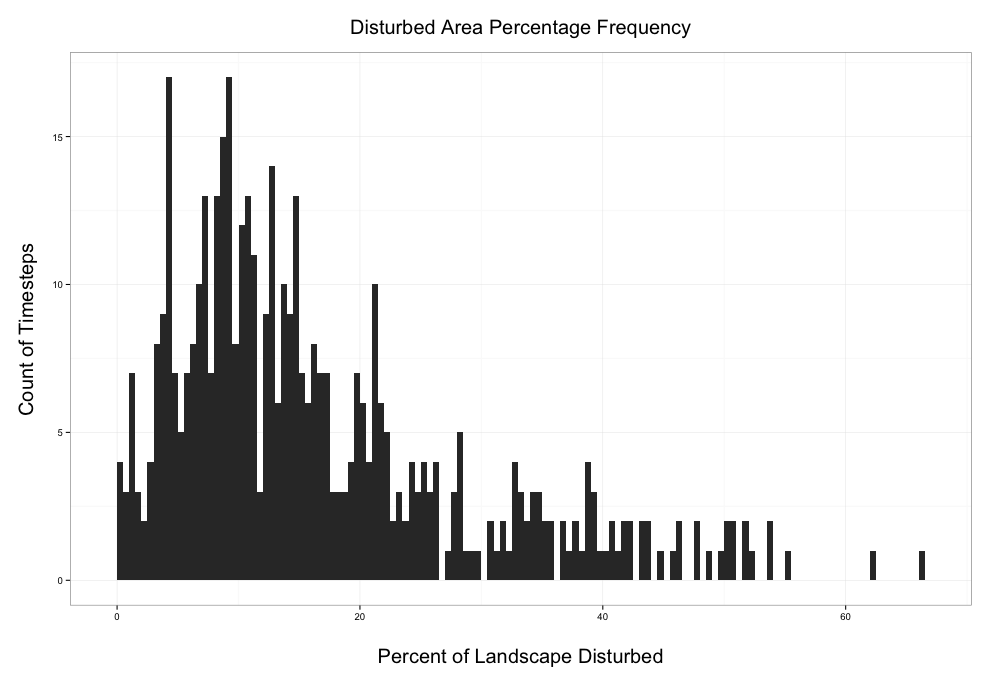
\includegraphics[width=0.6\textwidth]{/Users/mmallek/Tahoe/Report2/images/darea_hist.png}
\caption{Histogram of percent of landscape disturbed by wildfire during the simulation. The distribution is substantially right-skewed, and most fires burn less than 20\% of the eligible landscape.}
\label{fig:darea_hist}
\end{figure}

% background color 24, 15, 41, 0
\todo{figures redone}
\begin{figure}[!htbp]
  \centering
  \subfloat[][]{
    \centering
    \includegraphics[width=0.5\textwidth]{/Users/mmallek/Tahoe/Report2/images/wfmort1250_min.png}
    \label{fig:darea_min}
  }%
  \subfloat[][]{
    \includegraphics[width=0.5\textwidth]{/Users/mmallek/Tahoe/Report2/images/distid1250_min.png}
    \label{fig:distid_min}
  }
  \caption{Maps of area burned during the timestep with the \textbf{least total area burned (0.72\%)} during the simulation. (a) Map by mortality level. Red indicates high mortality fire, while orange indicates low mortality fire. (b) Map showing each individual fire in a different color.}
  \label{fig:darea_min_map}
\end{figure}

\begin{figure}[!htbp]
  \centering
  \subfloat[][]{
    \centering
    \includegraphics[width=0.5\textwidth]{/Users/mmallek/Tahoe/Report2/images/wfmort1340_max.png}
    \label{fig:darea_max}
  }%
  \subfloat[][]{
    \includegraphics[width=0.5\textwidth]{/Users/mmallek/Tahoe/Report2/images/distid1340_max.png}
    \label{fig:distid_max}
  }
  \caption{Maps of area burned during the timestep with the \textbf{most total area burned (72.39\%)} during the simulation. (a) Map by mortality level. Red indicates high mortality fire, while orange indicates low mortality fire. (b) Map showing each individual fire in a different color.}
  \label{fig:darea_max_map}
\end{figure}

\begin{figure}[!htbp]
  \centering
  \subfloat[][]{
    \centering
    \includegraphics[width=0.5\textwidth]{/Users/mmallek/Tahoe/Report2/images/wfmort1945_median.png}
    \label{fig:darea_median}
  }%
  \subfloat[][]{
    \includegraphics[width=0.5\textwidth]{/Users/mmallek/Tahoe/Report2/images/distid1945_median.png}
    \label{fig:distid_median}
  }
  \caption{Maps of area burned during the timestep with the \textbf{median total area burned (14.28\%)} during the simulation. (a) Map by mortality level. Red indicates high mortality fire, while orange indicates low mortality fire. (b) Map showing each individual fire in a different color.}
  \label{fig:darea_median_map}
\end{figure}

\begin{figure}[!htbp]
  \centering
  \subfloat[][]{
    \centering
    \includegraphics[width=0.5\textwidth]{/Users/mmallek/Tahoe/Report2/images/wfmort940_mean.png}
    \label{fig:darea_mean}
  }%
  \subfloat[][]{
    \includegraphics[width=0.5\textwidth]{/Users/mmallek/Tahoe/Report2/images/distid940_mean.png}
    \label{fig:distid_mean}
  }
  \caption{Maps of area burned during the timestep with the \textbf{mean total area burned (17.53\%)} during the simulation. (a) Map by mortality level. Red indicates high mortality fire, while orange indicates low mortality fire. (b) Map showing each individual fire in a different color.}
  \label{fig:darea_mean_map}
\end{figure}

\subsubsection{Disturbance Size} \todo{repaired}
As described in Section \ref{subsubsec:distparams}, we specified a target set of disturbance sizes. Because wildfire has many stochastic components, we do not expect the model results to match these targets exactly. Figure \ref{fig:dsize} compares the observed and target disturbance size distribution.



\begin{figure}[!htbp]
\centering
\includegraphics[width=0.7\textwidth]{/Users/mmallek/Tahoe/R/Rplots/November2014/dsize.png}
\caption{Side by side barplot of the observed and target wildfire size distribution for our 500-timestep long run of the model.}
\label{fig:dsize}
\end{figure}



\subsubsection{Effect of Climate} \todo{repaired, except for dsize related plots, since it appears they were never working correctly - not sure if problem is dsize data or plotting}
Climate does have a positive relationship with disturbed area, as expected (Figure \ref{fig:climate_darea}. We show here a fitted line, but note the heteroskedastic variance about the mean. The relationship is fairly weak. During wetter-than-average years, we see less disturbed area. Over 20\% of the landscape burned only in timesteps during which the climate parameter was at least 0.63. However, over 50\% of the landscape burned in several timesteps when the climate parameter was less than 1, which is the average value over the historical period. Overall we observe that as climate shifts from wet to drought, the disturbed area increases. %Climate also has a weak effect on the size of individual fires (Figure \ref{fig:climate_dsize}). 
Fire size is also influenced by vegetation susceptibility and the specified disturbance size distribution. For this reason, large areas may burn in relatively ``wet'' years. Figure \ref{fig:compare_clim_darea} illustrates the climate parameter values and disturbed area proportion of the landscape for a subset of timesteps during the simulation.
\todo{the dsize function has something wrong with it (and always did)}
\begin{figure}[!htbp]
  \centering
  \subfloat[][]{
    \centering
    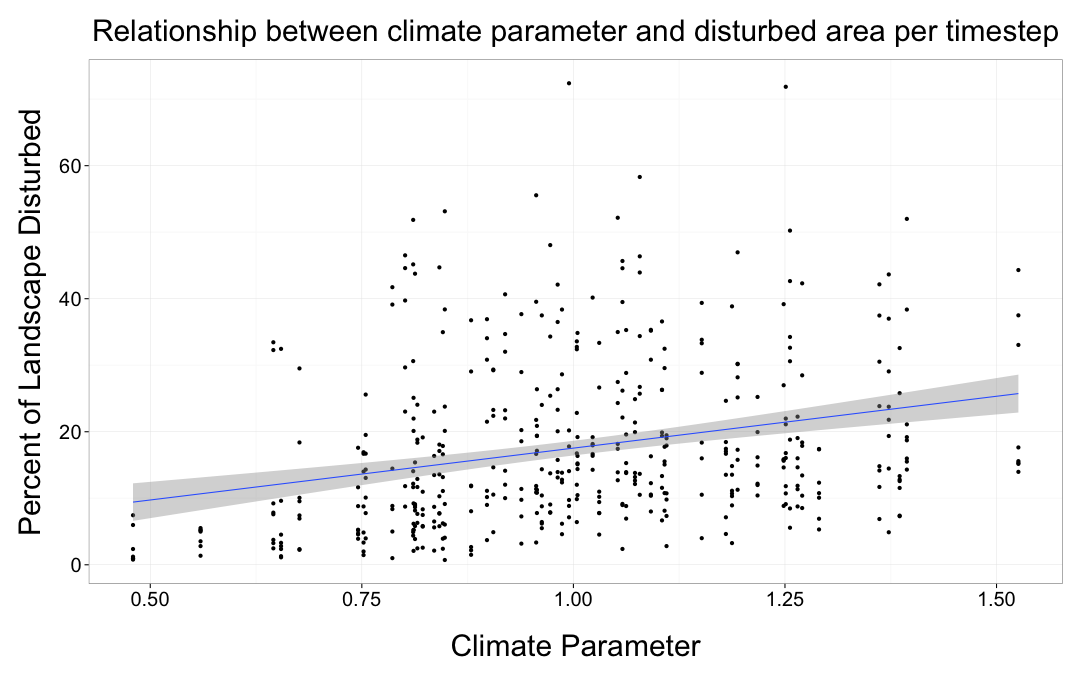
\includegraphics[width=0.7\textwidth]{/Users/mmallek/Tahoe/Report2/images/climate_darea.png}
    \label{fig:climate_darea}
  }%
  %\qquad
 % \subfloat[][]{
 %   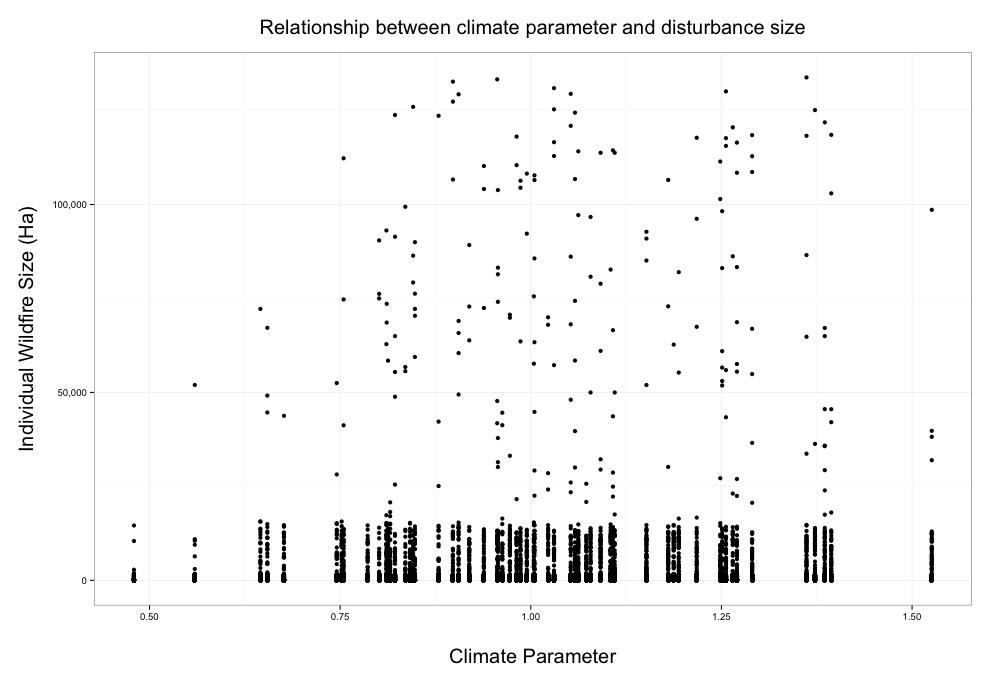
\includegraphics[width=0.5\textwidth]{/Users/mmallek/Tahoe/Report2/images/climate_dsize.png}
 %   \label{fig:climate_dsize}
 % }
  %\caption{(a) Plot of the climate parameter and disturbed area value for each timestep of the simulation (excluding the  equilibration period). A linear model has been fit to the data and is shown as a blue line; the grey shaded area represents  the 95\% confidence interval around the mean. (b) Plot showing the size of each individual wildfire and the climate parameter value in effect at the time of disturbance for each disturbance during the simulation (excluding the equilibration period).}
    \caption{Plot of the climate parameter and disturbed area value for each timestep of the simulation (excluding the  equilibration period). A linear model has been fit to the data and is shown as a blue line; the grey shaded area represents  the 95\% confidence interval around the mean.}
  \label{fig:climate_disturbance}
\end{figure}

\begin{figure}[!htbp]
\centering
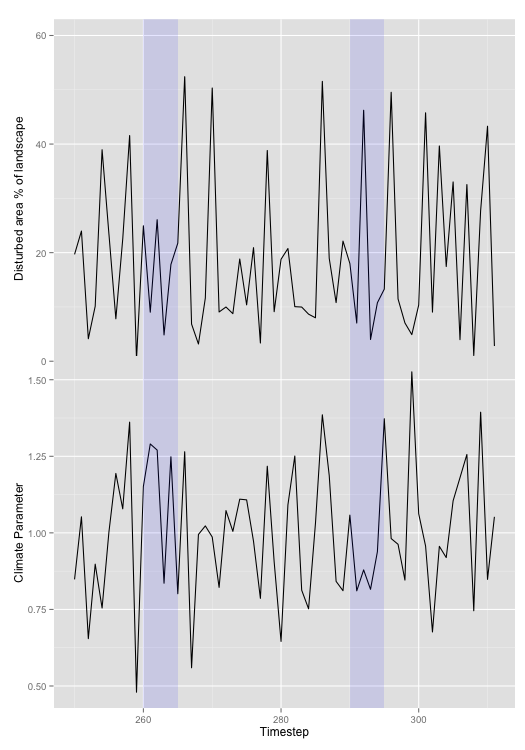
\includegraphics[width=0.8\textwidth]{/Users/mmallek/Tahoe/Report2/images/climate_darea_vert.png}
\caption{Climate parameter and proportion of eligible landscape disturbed by wildfire for timesteps 250 to 310 of the simulation.}
\label{fig:compare_clim_darea}
\end{figure}

\clearpage
\subsubsection{Effect of Topographic Position}\todo{redone}

The topographic position index value for a given cell acts as an input into the susceptibility and mortality values otherwise defined for that cover type and condition class combination. In general, cells with smaller TPI values had reduced susceptibility and mortality. Early development and open canopy conditions tend to result from fire, and we predicted that an increase in fires and in the likelihood of high mortality fire would lead to a decrease in the average canopy cover values for cells with large TPI values. Table \ref{tab:tpi_cc} displays the results for this simulation for the nine focal cover types. All but the mixed evergreen types show decreased average canopy cover as TPI increases, with the decrease ranging from 6.2\% in Oak-Conifer Forest and Woodland to 32.4\% in Red Fir - Xeric. Figure \ref{fig:tpi_cc} shows the plotted data and fitted linear regression line for each of the nine focal types. Figure \ref{fig:averagecc} is a map displaying average canopy cover across the landscape for the full simulated HRV timeframe, excluding the equilibration period. 

\begin{figure}[!htbp]
\centering
\includegraphics[width=0.8\textwidth]{/Users/mmallek/Tahoe/Report2/images/averagecc.jpg}
\caption{Smoothed visualization of the average canopy cover across the project area over the course of the simulation. Higher percent cover is shown in blue, transitioning to red where average percent cover was low.}
\label{fig:averagecc}
\end{figure}

\begin{table}[!htbp]
\caption{For each cover type on the landscape, the percent change in canopy cover from the minimum TPI value for that cover type to the maximum TPI value.}
\label{tab:tpi_cc}
%\rotatebox{90}{
\begin{tabular}{@{}lrrrrr@{}}
\toprule
\small \textbf{\begin{tabular}[c]{@{}l@{}}Cover \\ Name\end{tabular}} & \small \textbf{\begin{tabular}[c]{@{}l@{}}Minimum \\ TPI\end{tabular}} & \small \textbf{\begin{tabular}[c]{@{}l@{}}Maximum \\ TPI\end{tabular}} & \small \textbf{\begin{tabular}[c]{@{}l@{}}Average Canopy \\Cover at \\ Minimum TPI\end{tabular}} & \small \textbf{\begin{tabular}[c]{@{}l@{}}Average Canopy \\ Cover at \\ Maximum TPI\end{tabular}}  & \small \textbf{\begin{tabular}[c]{@{}l@{}}Percent \\ Change in \\ Canopy \\ Cover\end{tabular}} \\ \midrule
\textsc{meg\_m   }    & -300                 & 300                  & 66.5         & 67.5              &  1.5      \\
\textsc{meg\_x   }    & -299                 & 300                  & 64.1         & 66.4              &  3.8      \\
\textsc{ocfw     }    & -300                 & 300                  & 49.6         & 46.5              &  -6.2      \\
\textsc{ocfw\_u  }    & -300                 & 300                  & 25.0         & 22.8              &  -9.0       \\
\textsc{rfr\_m   }    & -300                 & 300                  & 65.2         & 58.9              &  -9.7     \\
\textsc{rfr\_x   }    & -259                 & 300                  & 49.0         & 33.0              & -32.4     \\
\textsc{smc\_m   }    & -300                 & 300                  & 48.8         & 42.6              & -12.6      \\
\textsc{smc\_u   }    & -300                 & 300                  & 36.7         & 28.3              & -22.7     \\
\textsc{smc\_x   }    & -300                 & 300                  & 35.9         & 26.9              & -24.9     \\ \bottomrule
\end{tabular}
%}
\end{table}

\begin{figure}[!htbp]
\centering
\includegraphics[width=\textwidth]{/Users/mmallek/Tahoe/Report2/images/TPI_cc_focaltypes.png}
\label{fig:tpi_cc_focaltypes}
\caption{Average canopy cover for the nine focal cover types during the simulated. Each blue point represents one pixel of an individual cover type on the landscape grid. The black line is the result of a linear regression fit to the data. Table \ref{tab:tpi_cc} provides the numerical representation of the shift from minimum to maximum TPI values for each cover type. (a) Mixed Evergreen - Mesic; (b) Mixed Evergreen - Xeric; (c) Oak-Conifer Forest and Woodland; (d) Oak-Conifer Forest and Woodland - Ultramafic; (e) Red Fir - Mesic; (f) Red Fir - Xeric; (g) Sierran Mixed Conifer - Mesic; (h) Sierran Mixed Conifer - Ultramafic; (i) Sierran Mixed Conifer - Xeric.}
\label{fig:tpi_cc}
\end{figure}


%\begin{figure}[!htbp]
%  \centering
%  \subfloat[][]{
%    \centering
%    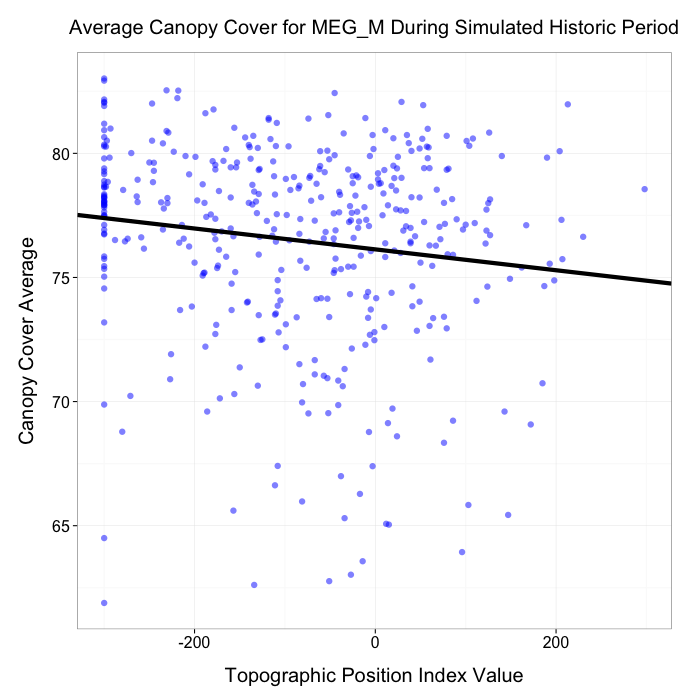
\includegraphics[width=0.33\textwidth]{/Users/mmallek/Tahoe/Report2/images/TPI_cc_megm.png}
%    \label{fig:tpi_cc_megm}
%  }%
%  \subfloat[][]{
%    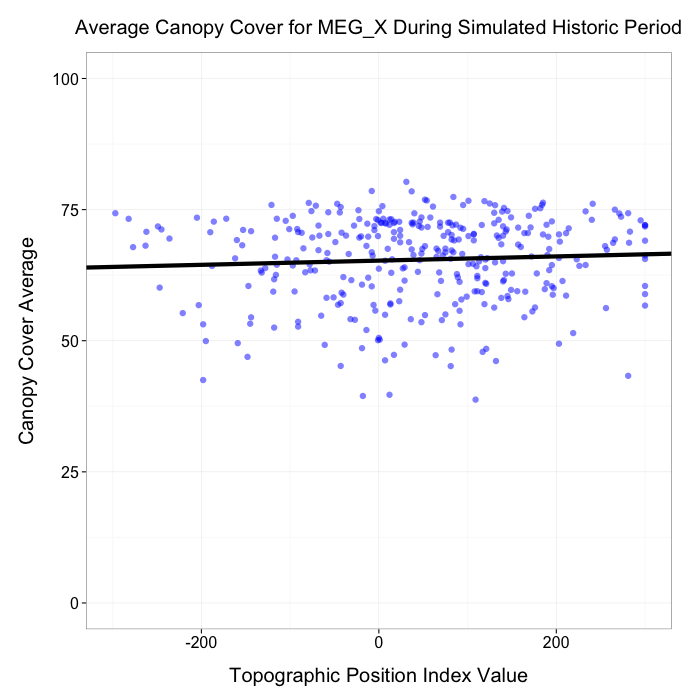
\includegraphics[width=0.33\textwidth]{/Users/mmallek/Tahoe/Report2/images/TPI_cc_megx.png}
%    \label{fig:tpi_cc_megx}
%  }%
%  \subfloat[][]{
%    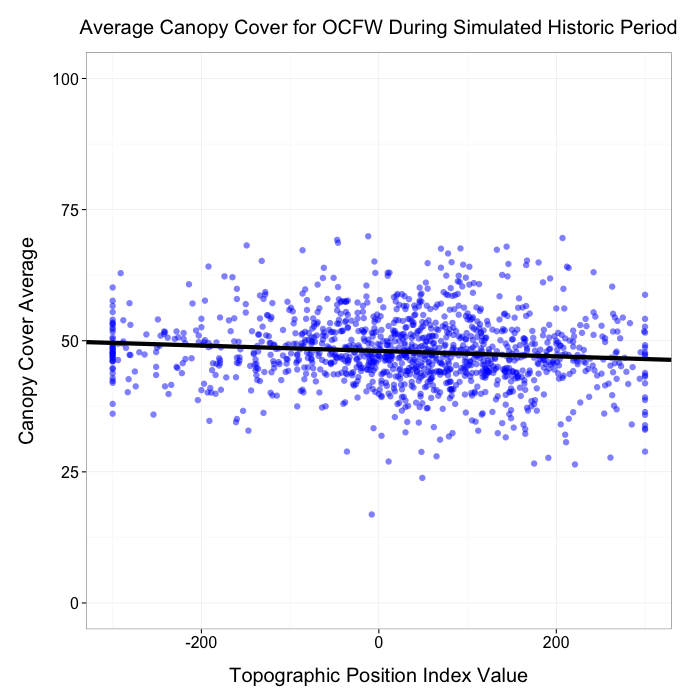
\includegraphics[width=0.33\textwidth]{/Users/mmallek/Tahoe/Report2/images/TPI_cc_ocfw.png}
%    \label{fig:ocfw}
%    }
%
%  \subfloat[][]{
%    \centering
%    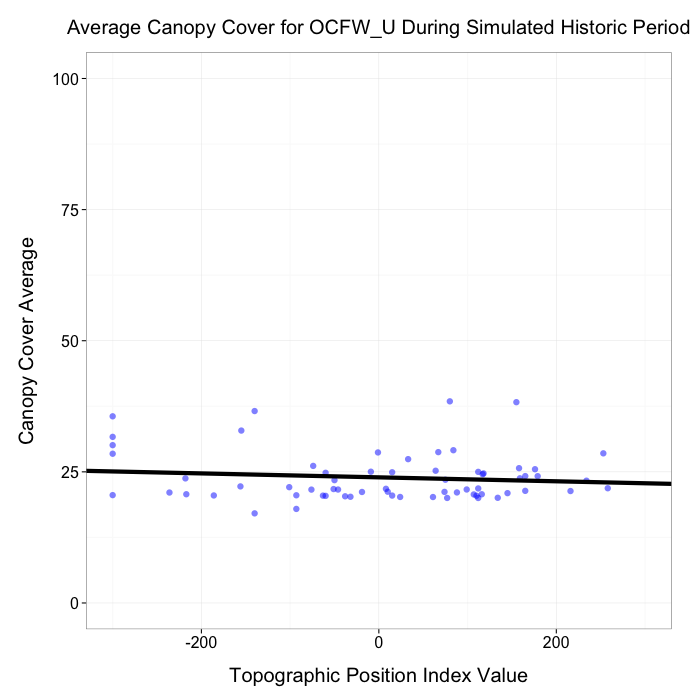
\includegraphics[width=0.33\textwidth]{/Users/mmallek/Tahoe/Report2/images/TPI_cc_ocfwu.png}
%    \label{fig:tpi_cc_ocfwu}
%  }%
%  \subfloat[][]{
%    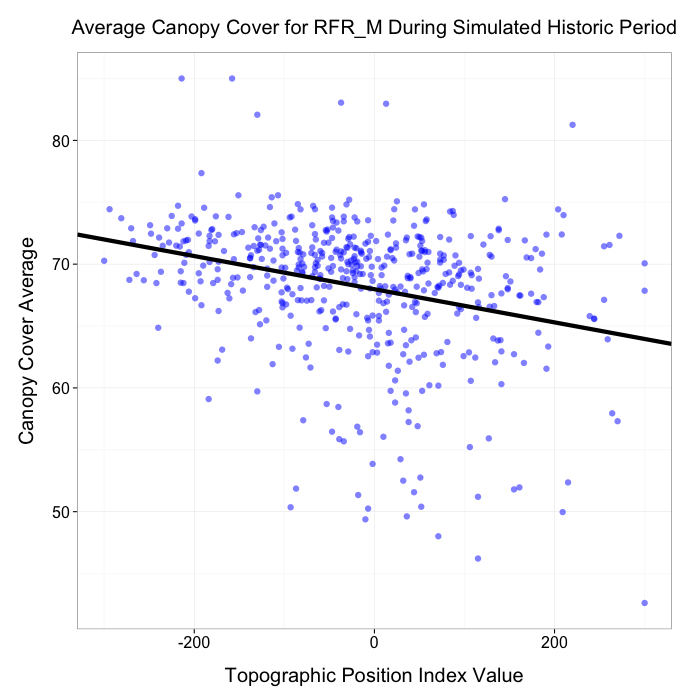
\includegraphics[width=0.33\textwidth]{/Users/mmallek/Tahoe/Report2/images/TPI_cc_rfrm.png}
%    \label{fig:tpi_cc_rfrm}
%  }%
%  \subfloat[][]{
%    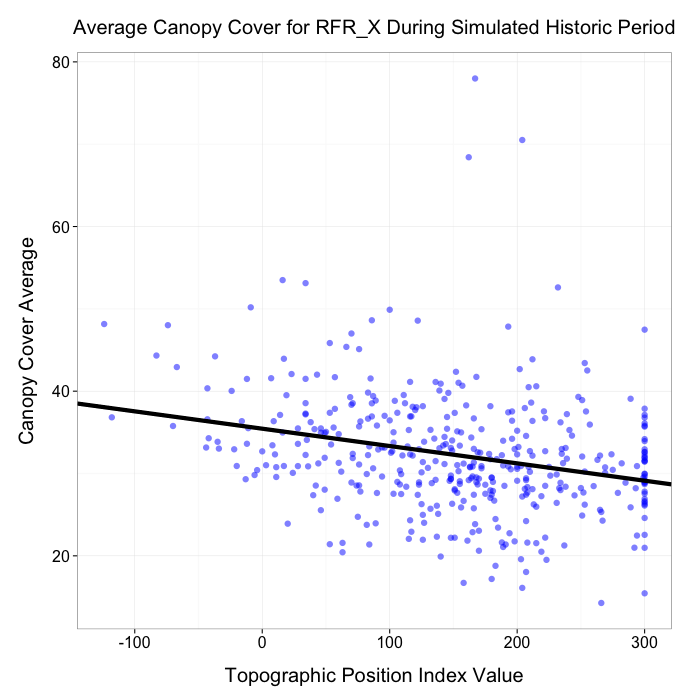
\includegraphics[width=0.33\textwidth]{/Users/mmallek/Tahoe/Report2/images/TPI_cc_rfrx.png}
%    \label{fig:tpi_cc_rfrx}
%    }
%
%  \subfloat[][]{
%    \centering
%    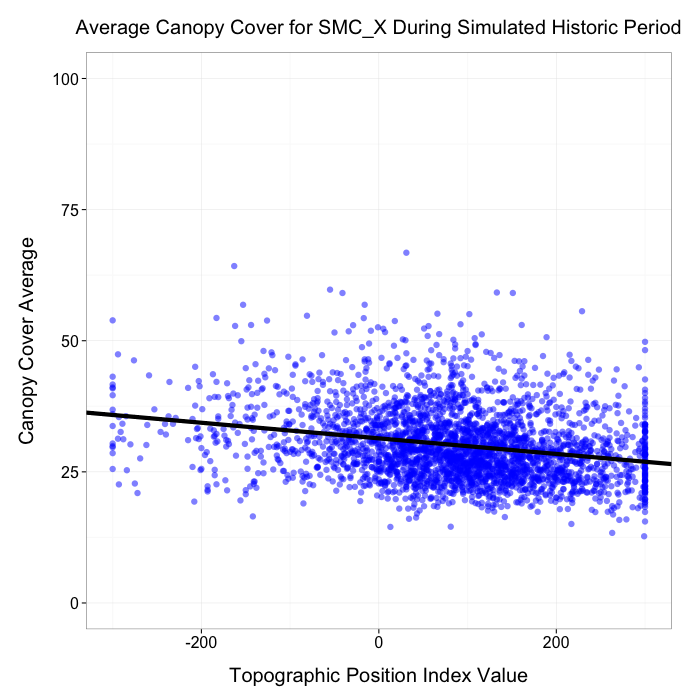
\includegraphics[width=0.33\textwidth]{/Users/mmallek/Tahoe/Report2/images/TPI_cc_smcx.png}
%    \label{fig:tpi_cc_smcm}
%  }%
%  \subfloat[][]{
%    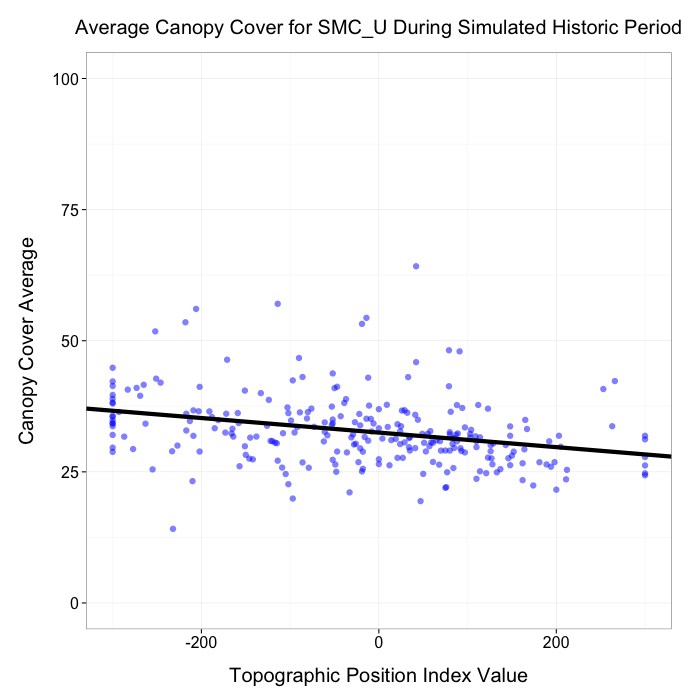
\includegraphics[width=0.33\textwidth]{/Users/mmallek/Tahoe/Report2/images/TPI_cc_smcu.png}
%    \label{fig:tpi_cc_smcu}
%  }%
%  \subfloat[][]{
%    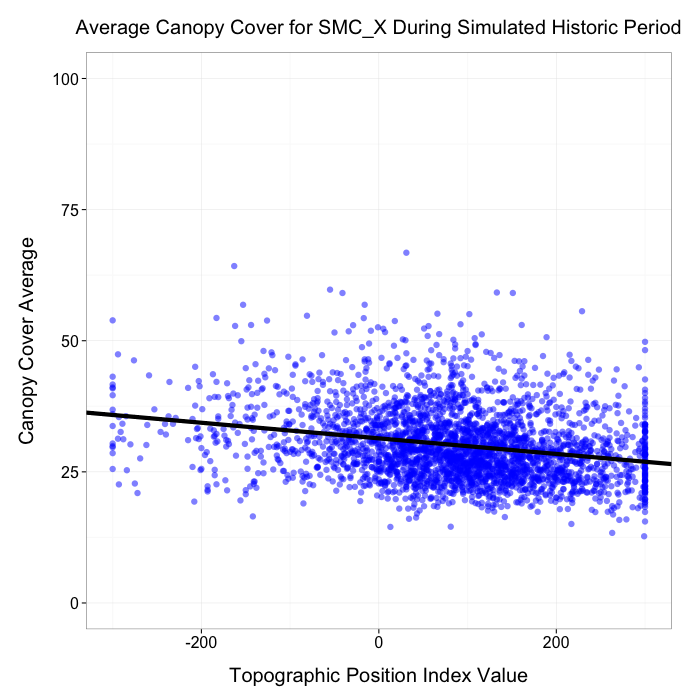
\includegraphics[width=0.33\textwidth]{/Users/mmallek/Tahoe/Report2/images/TPI_cc_smcx.png}
%    \label{fig:tpi_cc_smcx}
%    }
%  \caption{Average canopy cover for the nine focal cover types during the simulated. Each blue point represents one pixel of an individual cover type on the landscape grid. The black line is the result of a linear regression fit to the data. Note, the $y$ axis is scaled differently across cover types in order to more easily focus on the data for each type. Table \ref{tab:tpi_cc} provides the numerical representation of the shift from minimum to maximum TPI values for each cover type. (a) Mixed Evergreen - Mesic; (b) Mixed Evergreen - Xeric; (c) Oak-Conifer Forest and Woodland; (d) Oak-Conifer Forest and Woodland - Ultramafic; (e) Red Fir - Mesic; (f) Red Fir - Xeric; (g) Sierran Mixed Conifer - Mesic; (h) Sierran Mixed Conifer - Ultramafic; (i) Sierran Mixed Conifer - Xeric.}
%  \label{fig:tpi_cc}
%\end{figure}



\newpage
\subsubsection{Fire Rotation} \todo{redone}
We present here the results for non-static cover types whose extent is at least 1000 ha. Full results are presented in Appendix \ref{sec:full-rot-results}. As previously discussed, these results could have been presented in the methods section. Each of the nine cover types shown here were calibrated to within 10\% of their target values, which were based on empirical published values and local expert opinion.
\todo{this has been updated}
\begin{table}[!htbp]
\centering
\caption{Fire rotation for the nine cover types whose extent cover at least 1000 ha.}
\begin{tabular}{@{}lrrr@{}}
\toprule
Land Cover Type                              & \begin{tabular}[c]{@{}l@{}}Low Mortality \\ Fire Rotation\end{tabular} & \begin{tabular}[c]{@{}l@{}}High Mortality \\ Fire Rotation\end{tabular} & \begin{tabular}[c]{@{}l@{}}All Fires \\ Rotation\end{tabular} \\ \midrule
\textsc{meg\_m   }    & 61                          & 525                          & 55                 \\
\textsc{meg\_x   }    & 47                          & 434                          & 42                 \\
\textsc{ocfw     }    & 30                          & 115                          & 24                 \\
\textsc{ocfw\_u  }    & 44                          & 1295                         & 43                 \\
\textsc{rfr\_m   }    & 102                         & 160                          & 62                 \\
\textsc{rfr\_x   }    & 62                          & 108                          & 39                 \\
\textsc{smc\_m   }    & 36                          & 125                          & 28                 \\
\textsc{smc\_u   }    & 94                          & 196                          & 63                 \\
\textsc{smc\_x   }    & 36                          & 64                           & 23                 \\
\emph{Total    }      & 41                          & 106                          & 30                 \\ \bottomrule
\end{tabular}
\end{table}


\subsubsection{Population Return Interval}
Overall, the point-specific return interval (grand mean) for all eligible cells ranged from 17 years to \textgreater 2500 years (cells that never burned during the simulation) for both classes of wildfire mortality (Figure \ref{fig:preturn}). The median return interval across all cover types was 42 years for low mortality fire, 111 year for high mortality fire, and 29 years for any fire. The population return interval plots and maps specific to each of the nine focal cover types follow (Figures \ref{fig:preturn_megm} through \ref{fig:preturn_smcx}). We compare the current landscape's seral stage distribution to the simulated distribution and compute the HRV departure index in Tables \ref{tab:covcond1} and \ref{tab:covcond2}.
\todo{updated preturn R plots but not arcmap plots - maybe can skip until post-presentation?}
\begin{figure}[!htbp]
  \centering
  \subfloat[][]{
    \centering
    \includegraphics[height=0.4\textheight]{/Users/mmallek/Tahoe/R/Rplots/November2014/preturn_all.png}
    \label{fig:preturn_plot}
  }%
  \qquad
  \subfloat[][]{
    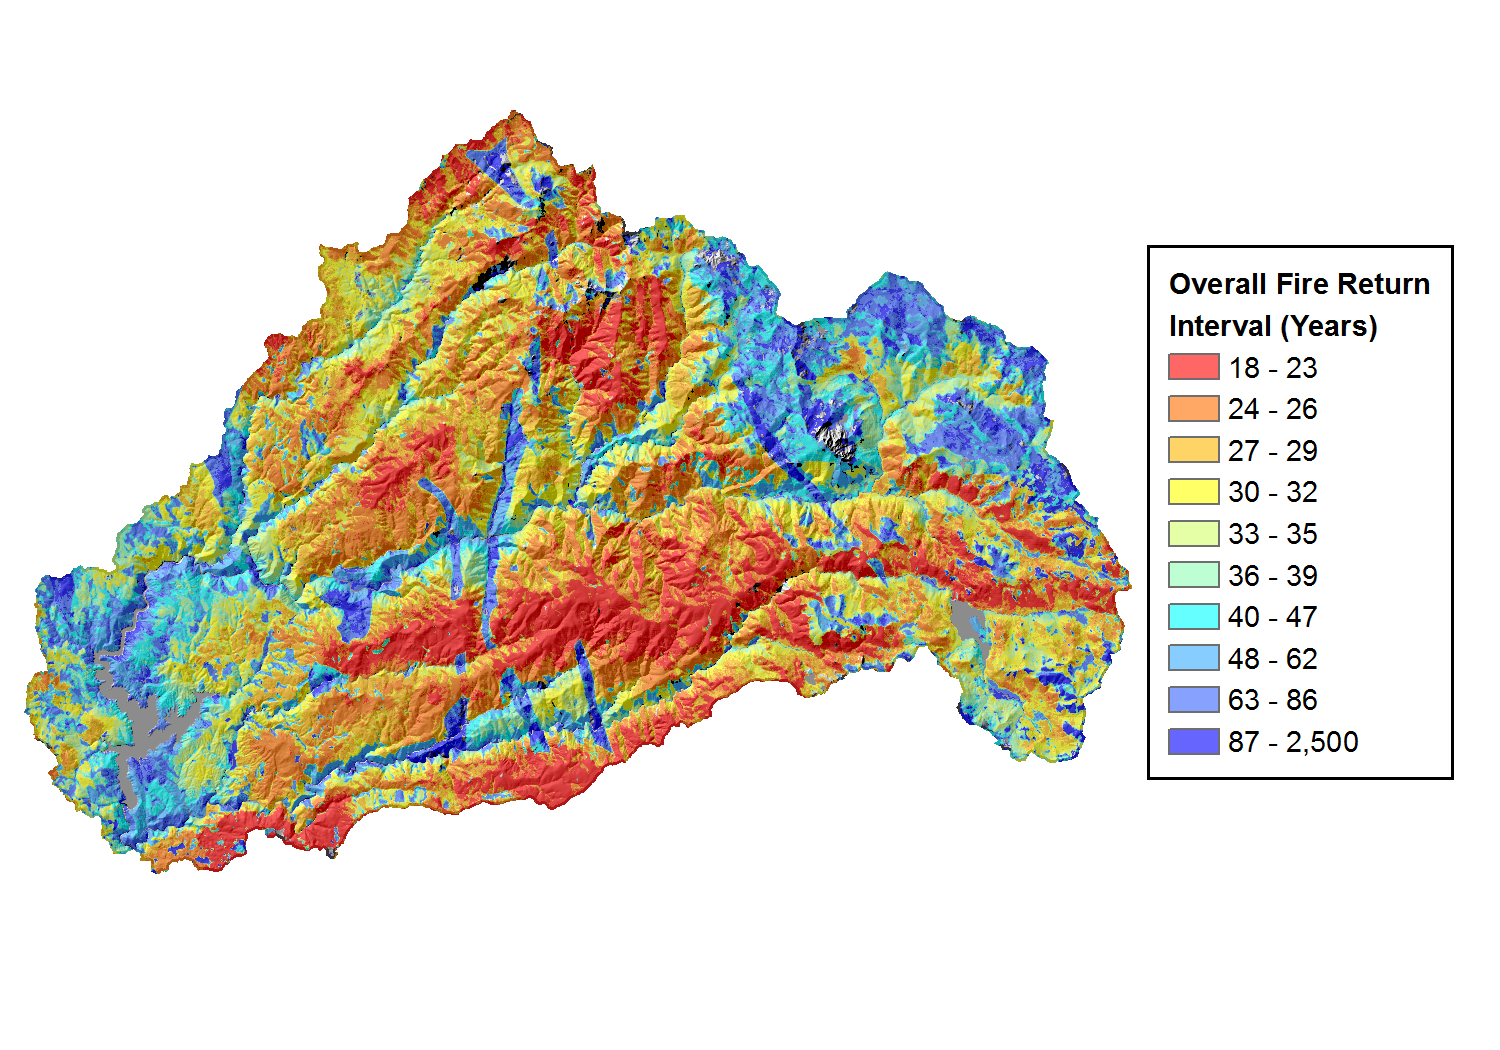
\includegraphics[height=0.4\textheight]{/Users/mmallek/Tahoe/Report2/images/fri_all.png}
    \label{fig:preturn_map}
  }
  \caption{(a) Population return interval (average number of years between fires) distribution for the full landscape under study. The population return interval is the point-specific interval, sometimes described as the ``grand mean'' for a given point. (b) Spatial depiction of fire return intervals across the landscape, for all cover types, in terms of fire return interval. The value at any given cell is the point-specific return interval.}
  \label{fig:preturn}
\end{figure}


\begin{figure}[!htbp]
  \centering
  \subfloat[][]{
    \centering
    \includegraphics[width=0.5\textwidth]{/Users/mmallek/Tahoe/R/Rplots/November2014/preturn_megm.png}
    }%
  \subfloat[][]{
    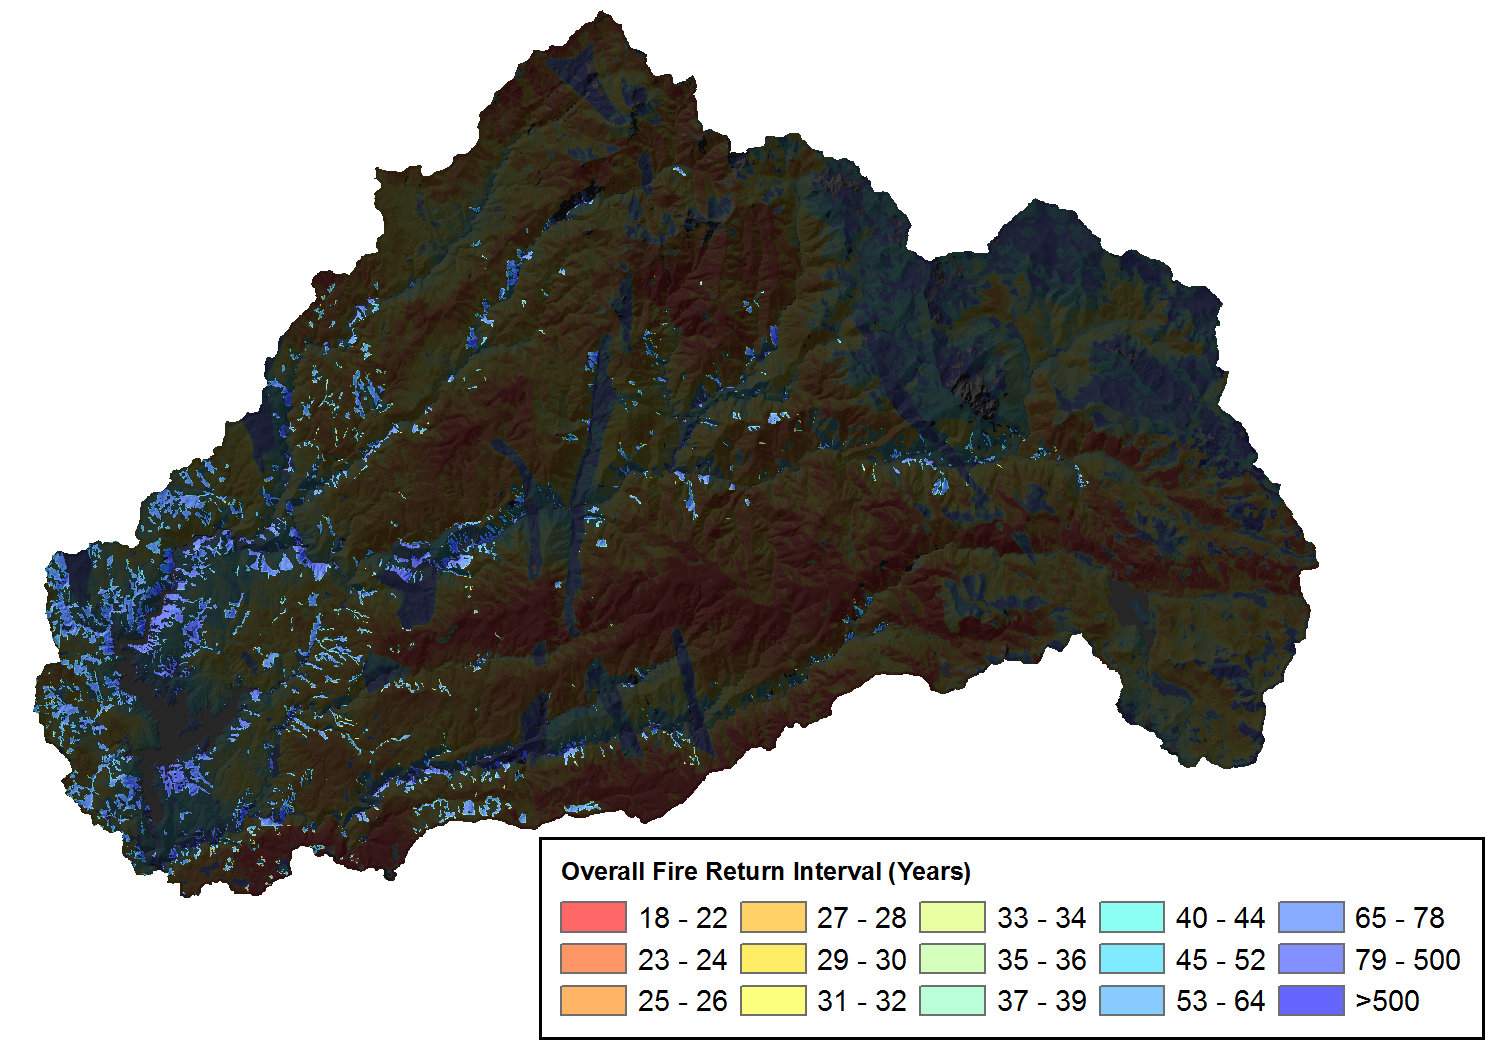
\includegraphics[width=0.5\textwidth]{/Users/mmallek/Tahoe/Report2/images/fri_megm.png}
    }
  \caption{(a) Population return interval (average number of years between fires) distribution for Mixed Evergreen - Mesic. (b) Spatial depiction of fire return intervals across the landscape. Cover types other than Mixed Evergreen - Mesic are partially obscured in grey. The value at any given cell is the point-specific return interval, which ranges from 20 years to \textgreater 500 years.}
    \label{fig:preturn_megm}
\end{figure}

\begin{figure}[!htbp]
  \centering
  \subfloat[][]{
    \centering
    \includegraphics[width=0.5\textwidth]{/Users/mmallek/Tahoe/R/Rplots/November2014/preturn_megx.png}
    }%
  \subfloat[][]{
    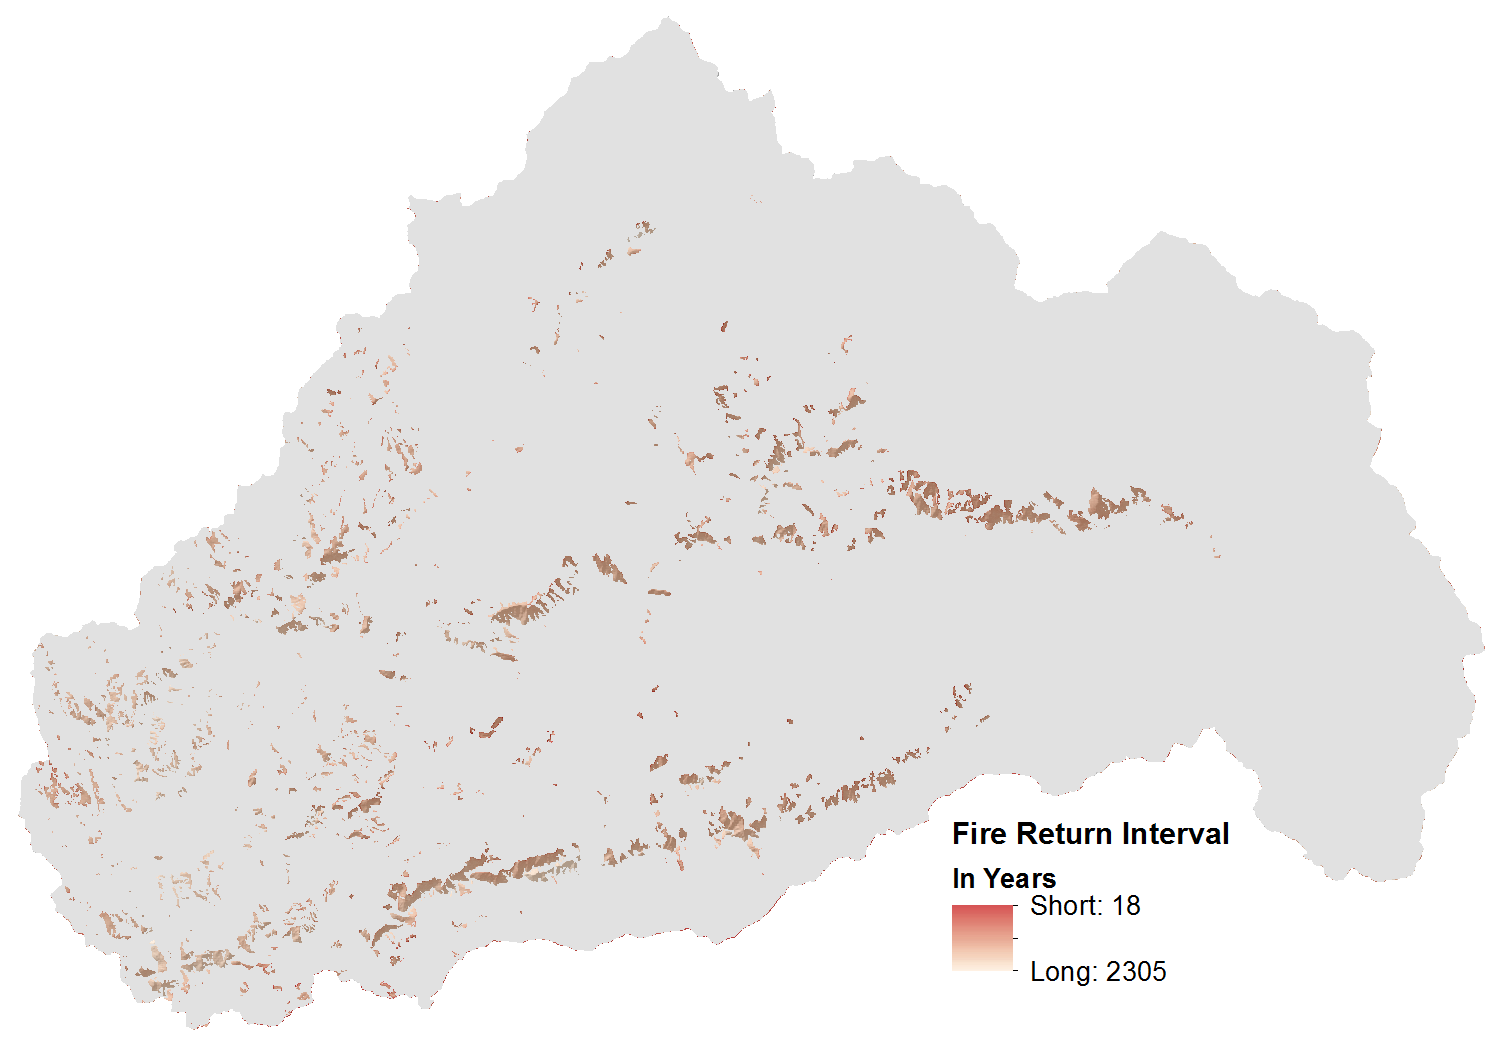
\includegraphics[width=0.5\textwidth]{/Users/mmallek/Tahoe/Report2/images/fri_megx.png}
    }
  \caption{(a) Population return interval (average number of years between fires) distribution for Mixed Evergreen - Xeric.  (b) Spatial depiction of fire return intervals across the landscape. Cover types other than Mixed Evergreen - Xeric are partially obscured in grey. The value at any given cell is the point-specific return interval, which ranges from 19 years to \textgreater 500 years.}
\label{fig:preturn_megx}
\end{figure}

\begin{figure}[!htbp]
  \centering
  \subfloat[][]{
    \centering
    \includegraphics[width=0.5\textwidth]{/Users/mmallek/Tahoe/R/Rplots/November2014/preturn_ocfw.png}
    }%
  \subfloat[][]{
    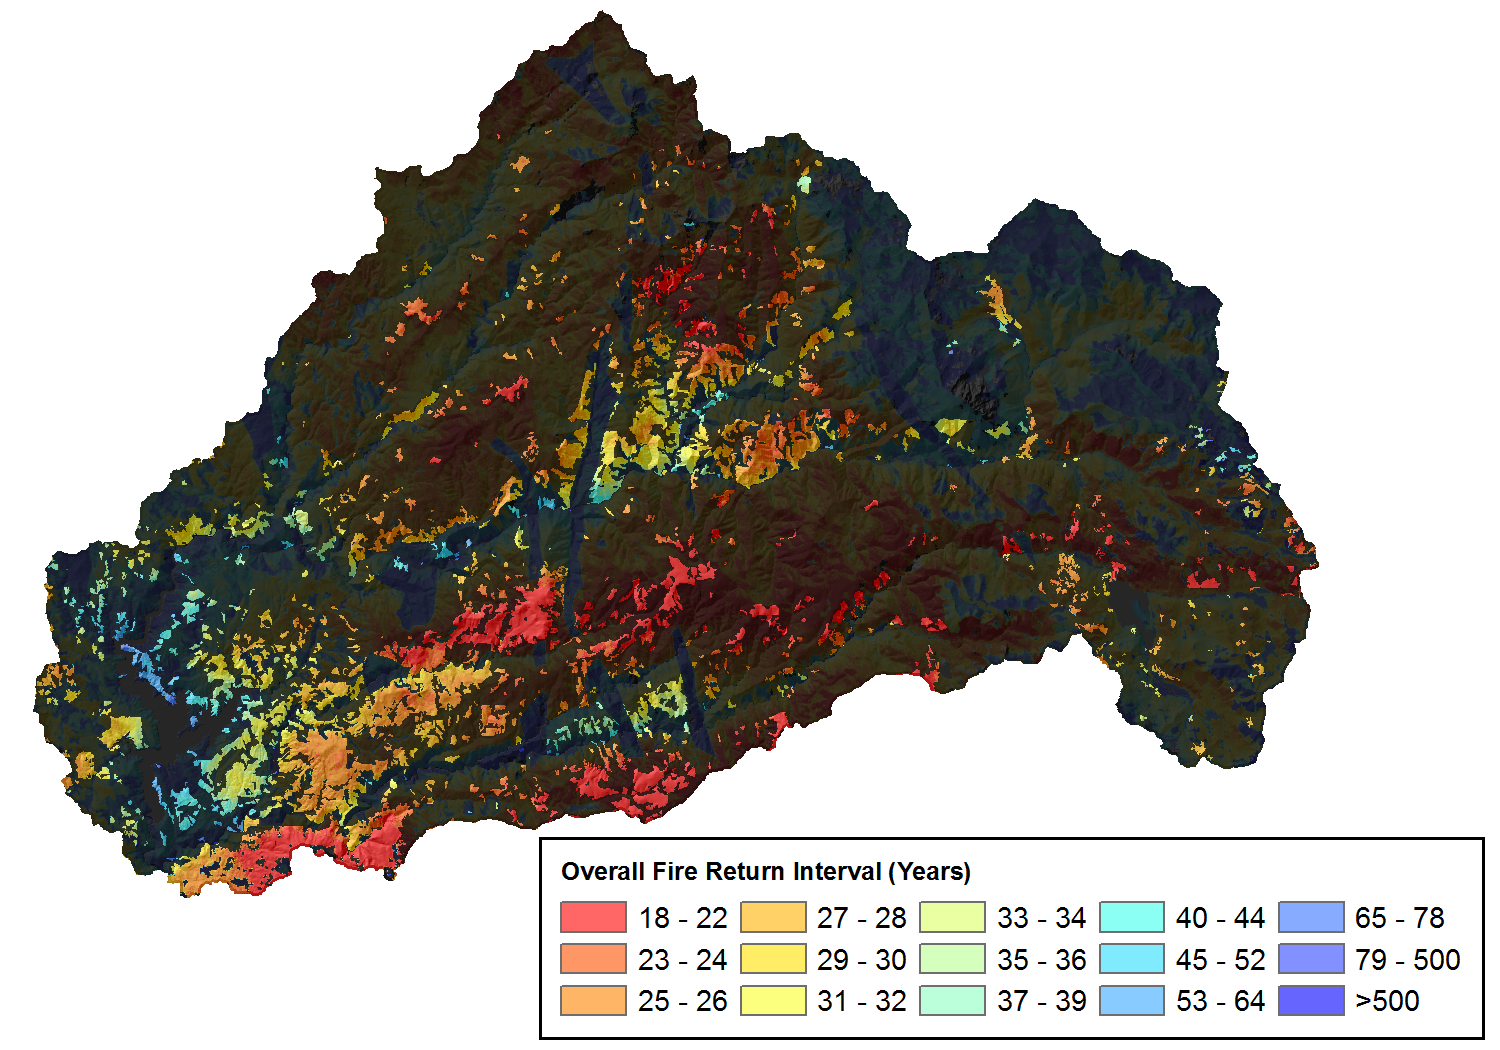
\includegraphics[width=0.5\textwidth]{/Users/mmallek/Tahoe/Report2/images/fri_ocfw.png}
    }
  \caption{(a) Population return interval (average number of years between fires) distribution for Oak-Conifer Forest and Woodland.  (b) Spatial depiction of fire return intervals across the landscape. Cover types other than Oak-Conifer Forest and Woodland are partially obscured in grey. The value at any given cell is the point-specific return interval, which ranges from 17 years to \textgreater 500 years.}
\label{fig:preturn_ocfw}
\end{figure}

\begin{figure}[!htbp]
  \centering
  \subfloat[][]{
    \centering
    \includegraphics[width=0.5\textwidth]{/Users/mmallek/Tahoe/R/Rplots/November2014/preturn_ocfwu.png}
    }%
  \subfloat[][]{
    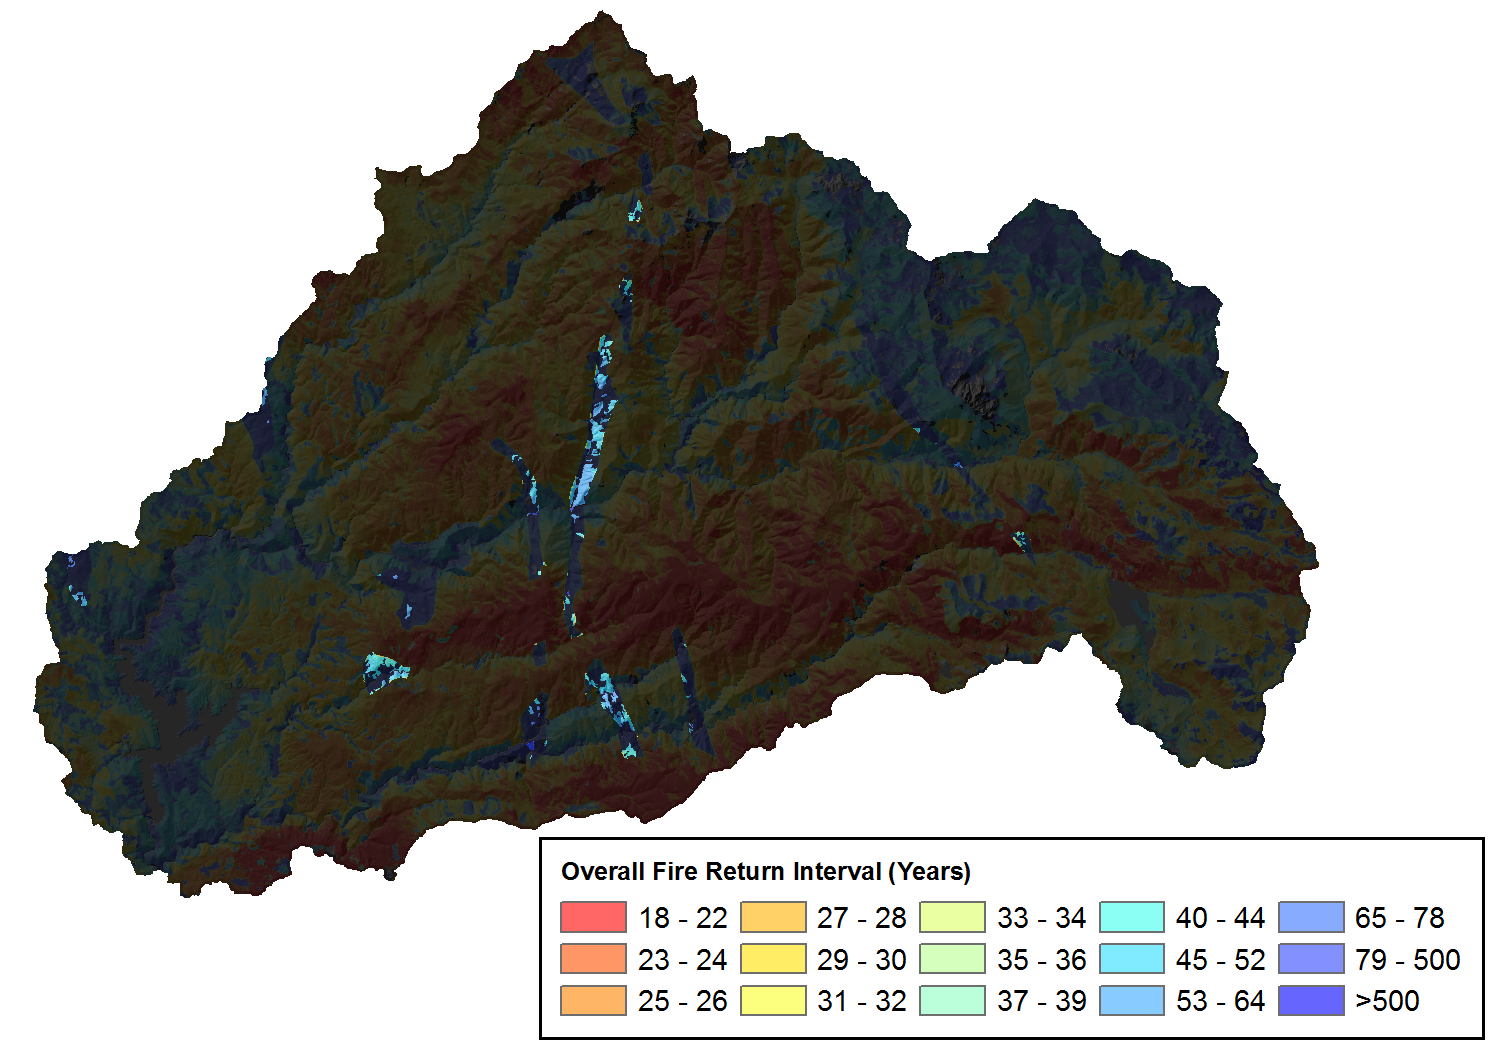
\includegraphics[width=0.5\textwidth]{/Users/mmallek/Tahoe/Report2/images/fri_ocfwu.png}
    }
  \caption{(a) Population return interval (average number of years between fires) distribution for Oak-Conifer Forest and Woodland - Ultramafic.  (b) Spatial depiction of fire return intervals across the landscape. Cover types other than Oak-Conifer Forest and Woodland - Ultramafic are partially obscured in grey. The value at any given cell is the point-specific return interval, which ranges from 20 years to \textgreater 500 years.}
\label{fig:preturn_ocfwu}
\end{figure}

\begin{figure}[!htbp]
  \centering
  \subfloat[][]{
    \centering
    \includegraphics[width=0.5\textwidth]{/Users/mmallek/Tahoe/R/Rplots/November2014/preturn_rfrm.png}
    }%
  \subfloat[][]{
    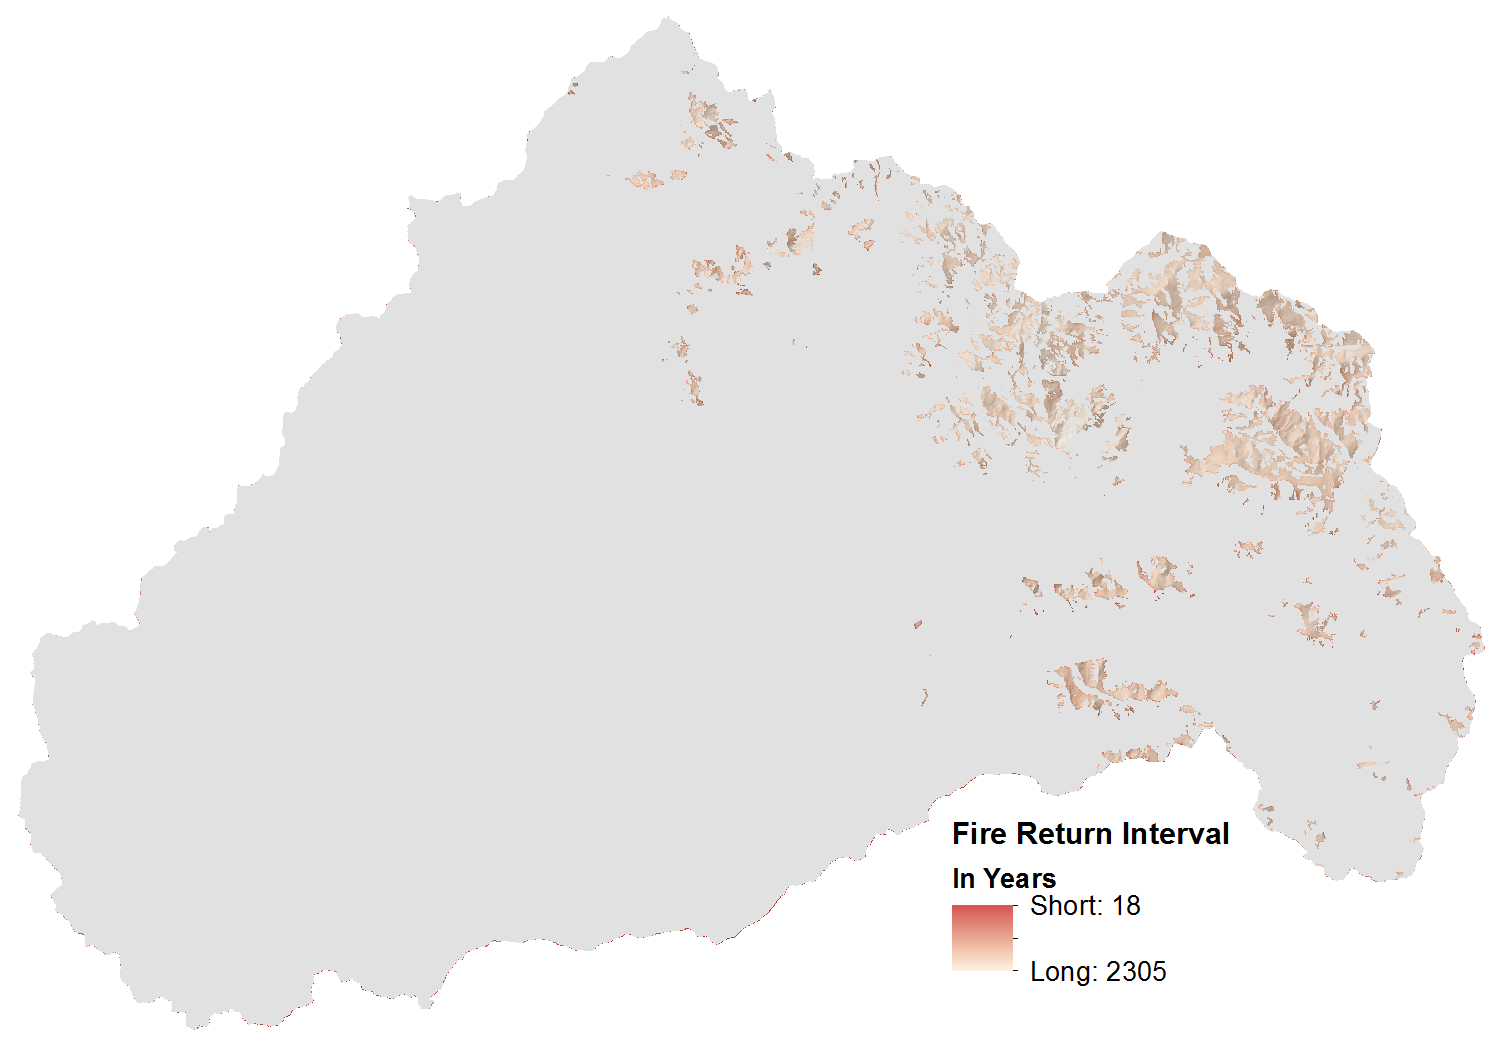
\includegraphics[width=0.5\textwidth]{/Users/mmallek/Tahoe/Report2/images/fri_rfrm.png}
    }
  \caption{(a) Population return interval (average number of years between fires) distribution for Red Fir - Mesic.  (b) Spatial depiction of fire return intervals across the landscape. Cover types other than Red Fir - Mesic are partially obscured in grey. The value at any given cell is the point-specific return interval, which ranges from 20 years to \textgreater 500 years.}
\label{fig:preturn_rfrm}
\end{figure}

\begin{figure}[!htbp]
  \centering
  \subfloat[][]{
    \centering
    \includegraphics[width=0.5\textwidth]{/Users/mmallek/Tahoe/R/Rplots/November2014/preturn_rfrx.png}
    }%
  \subfloat[][]{
    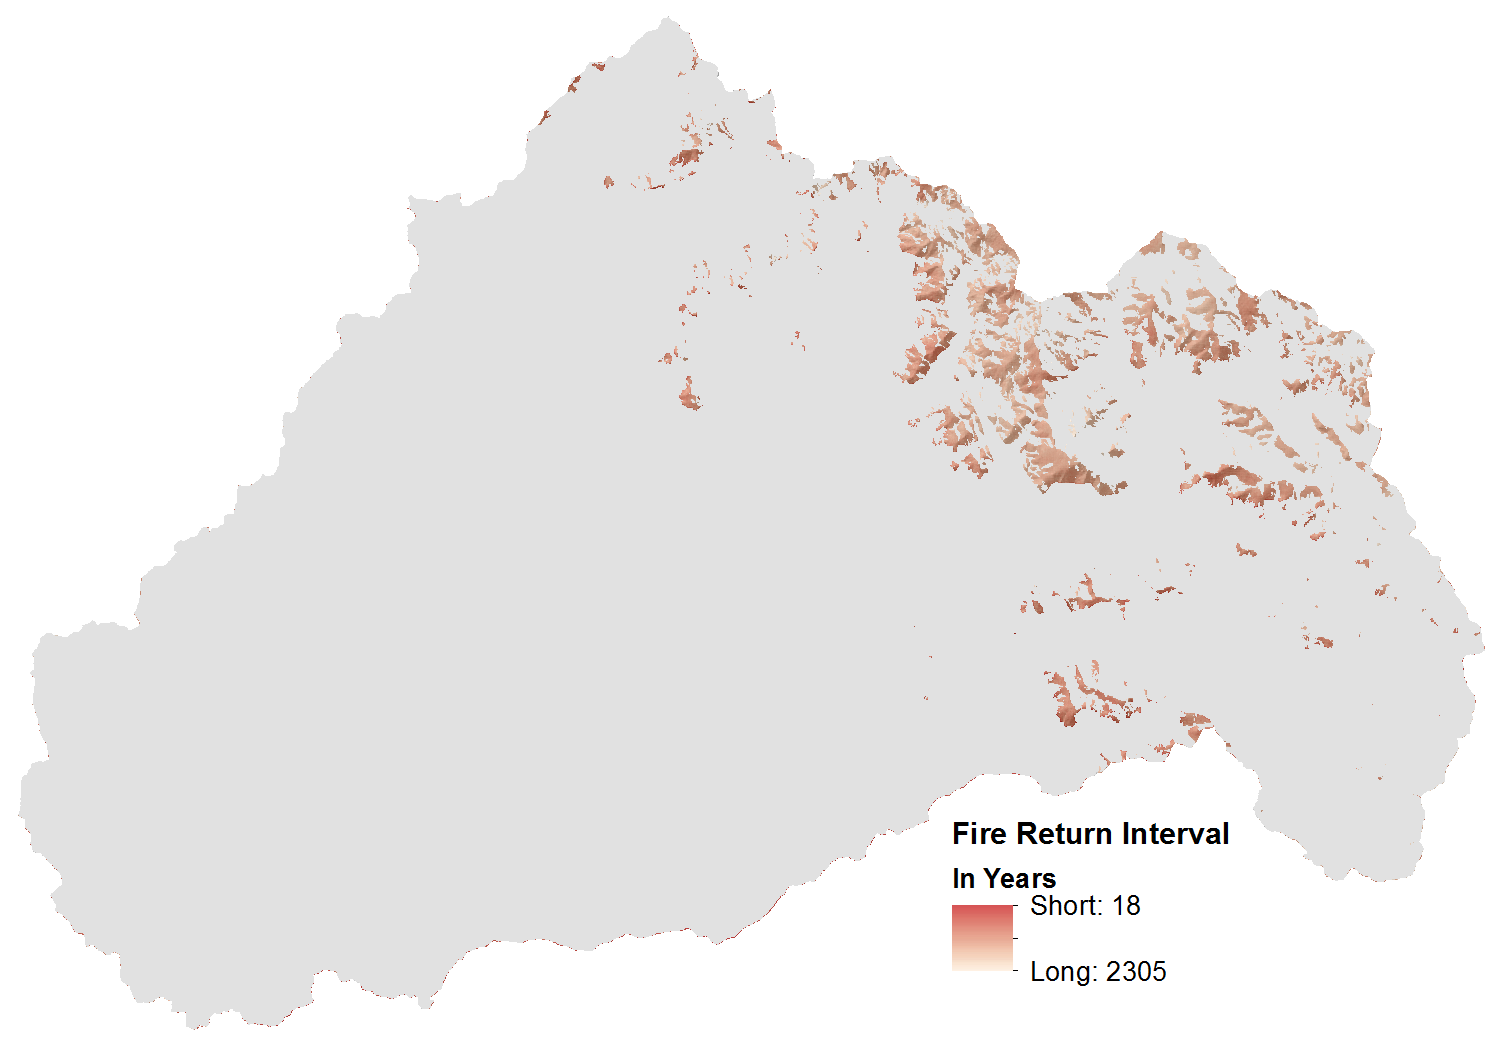
\includegraphics[width=0.5\textwidth]{/Users/mmallek/Tahoe/Report2/images/fri_rfrx.png}
    }
  \caption{(a) Population return interval (average number of years between fires) distribution for Red Fir - Xeric.  (b) Spatial depiction of fire return intervals across the landscape. Cover types other than Red Fir - Xeric are partially obscured in grey. The value at any given cell is the point-specific return interval, which ranges from 19 years to \textgreater 500 years.}
\label{fig:preturn_rfrx}
\end{figure}

\begin{figure}[!htbp]
  \centering
  \subfloat[][]{
    \centering
    \includegraphics[width=0.5\textwidth]{/Users/mmallek/Tahoe/R/Rplots/November2014/preturn_smcm.png}
    }%
  \subfloat[][]{
    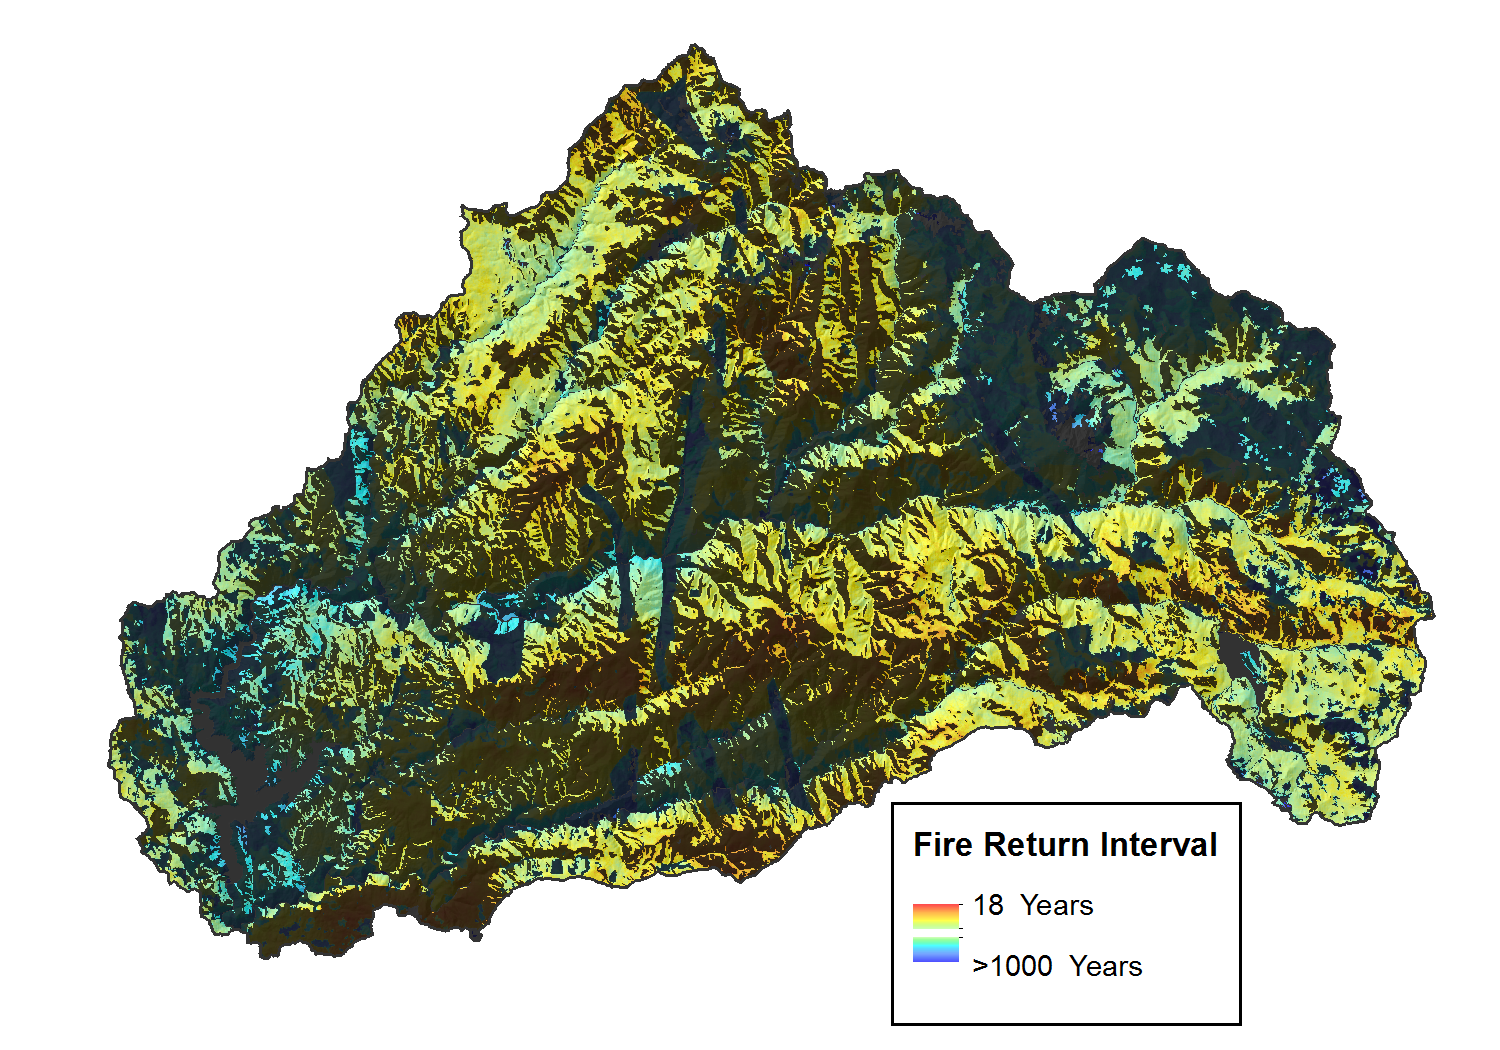
\includegraphics[width=0.5\textwidth]{/Users/mmallek/Tahoe/Report2/images/fri_smcm.png}
    }
  \caption{(a) Population return interval (average number of years between fires) distribution for Sierran Mixed Conifer - Mesic.  (b) Spatial depiction of fire return intervals across the landscape. Cover types other than Sierran Mixed Conifer - Mesic are partially obscured in grey. The value at any given cell is the point-specific return interval, which ranges from 18 years to \textgreater 500 years.}
\label{fig:preturn_smcm}
\end{figure}

\begin{figure}[!htbp]
  \centering
  \subfloat[][]{
    \centering
    \includegraphics[width=0.5\textwidth]{/Users/mmallek/Tahoe/R/Rplots/November2014/preturn_smcu.png}
    }%
  \subfloat[][]{
    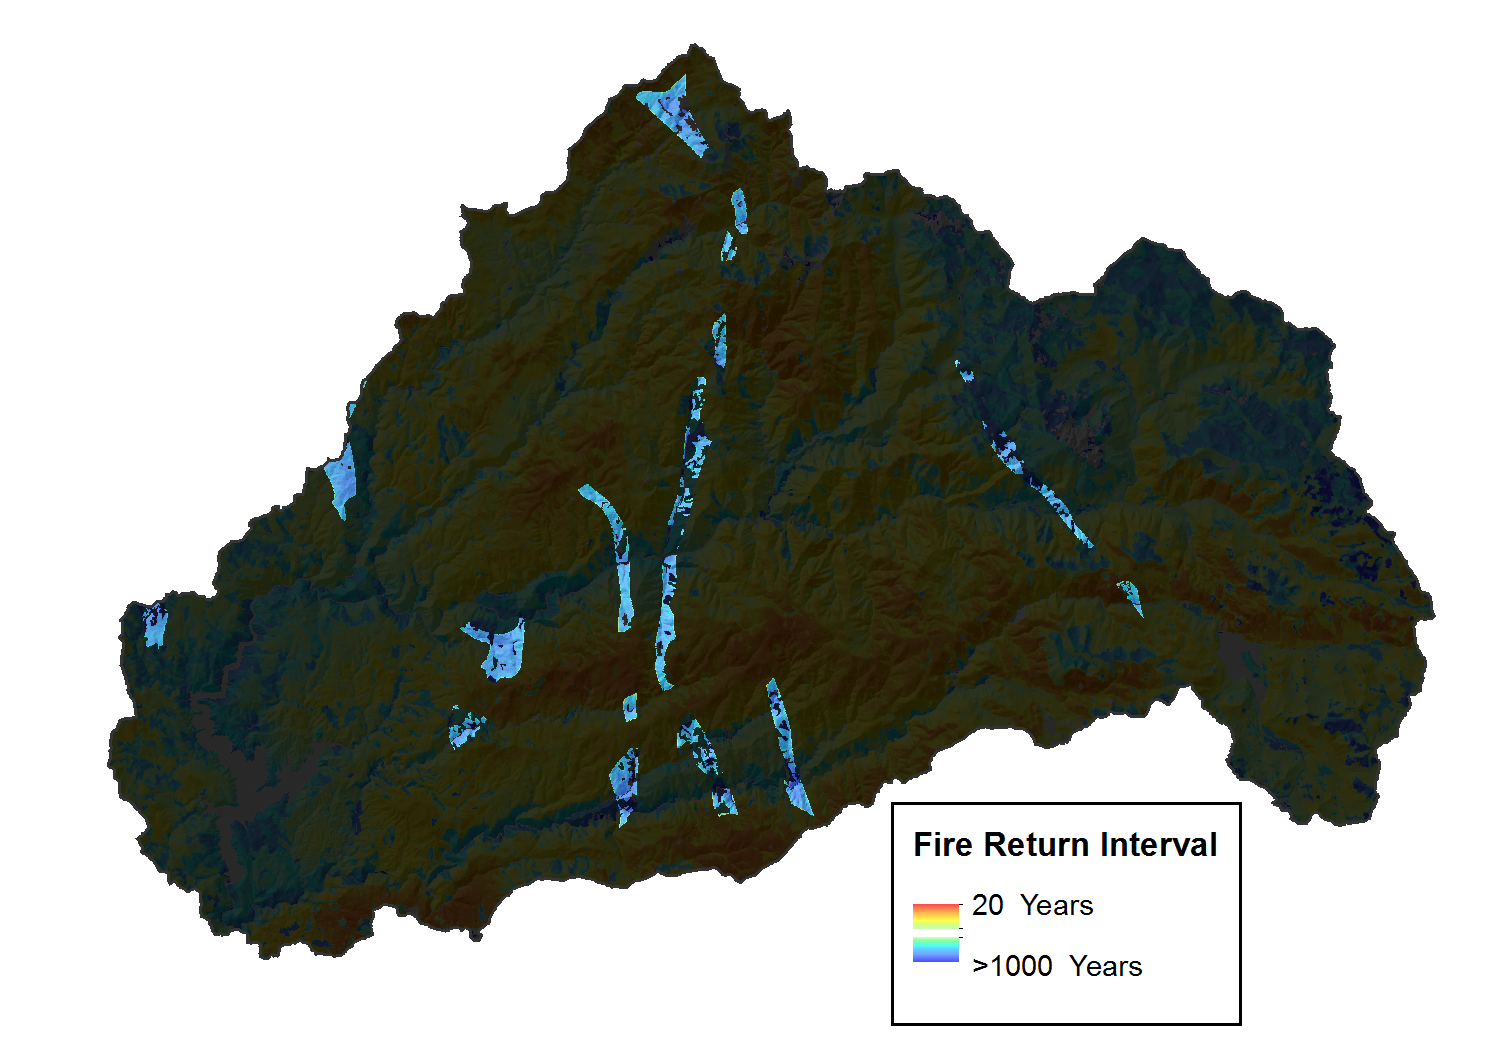
\includegraphics[width=0.5\textwidth]{/Users/mmallek/Tahoe/Report2/images/fri_smcu.png}
    }
  \caption{(a) Population return interval (average number of years between fires) distribution for Sierran Mixed Conifer - Ultramafic.  (b) Spatial depiction of fire return intervals across the landscape. Cover types other than Sierran Mixed Conifer - Ultramafic are partially obscured in grey. The value at any given cell is the point-specific return interval, which ranges from 21 years to \textgreater 500 years.}
\label{fig:preturn_smcu}
\end{figure}

\begin{figure}[!htbp]
  \centering
  \subfloat[][]{
    \centering
    \includegraphics[width=0.5\textwidth]{/Users/mmallek/Tahoe/R/Rplots/November2014/preturn_smcx.png}
    }%
  \subfloat[][]{
    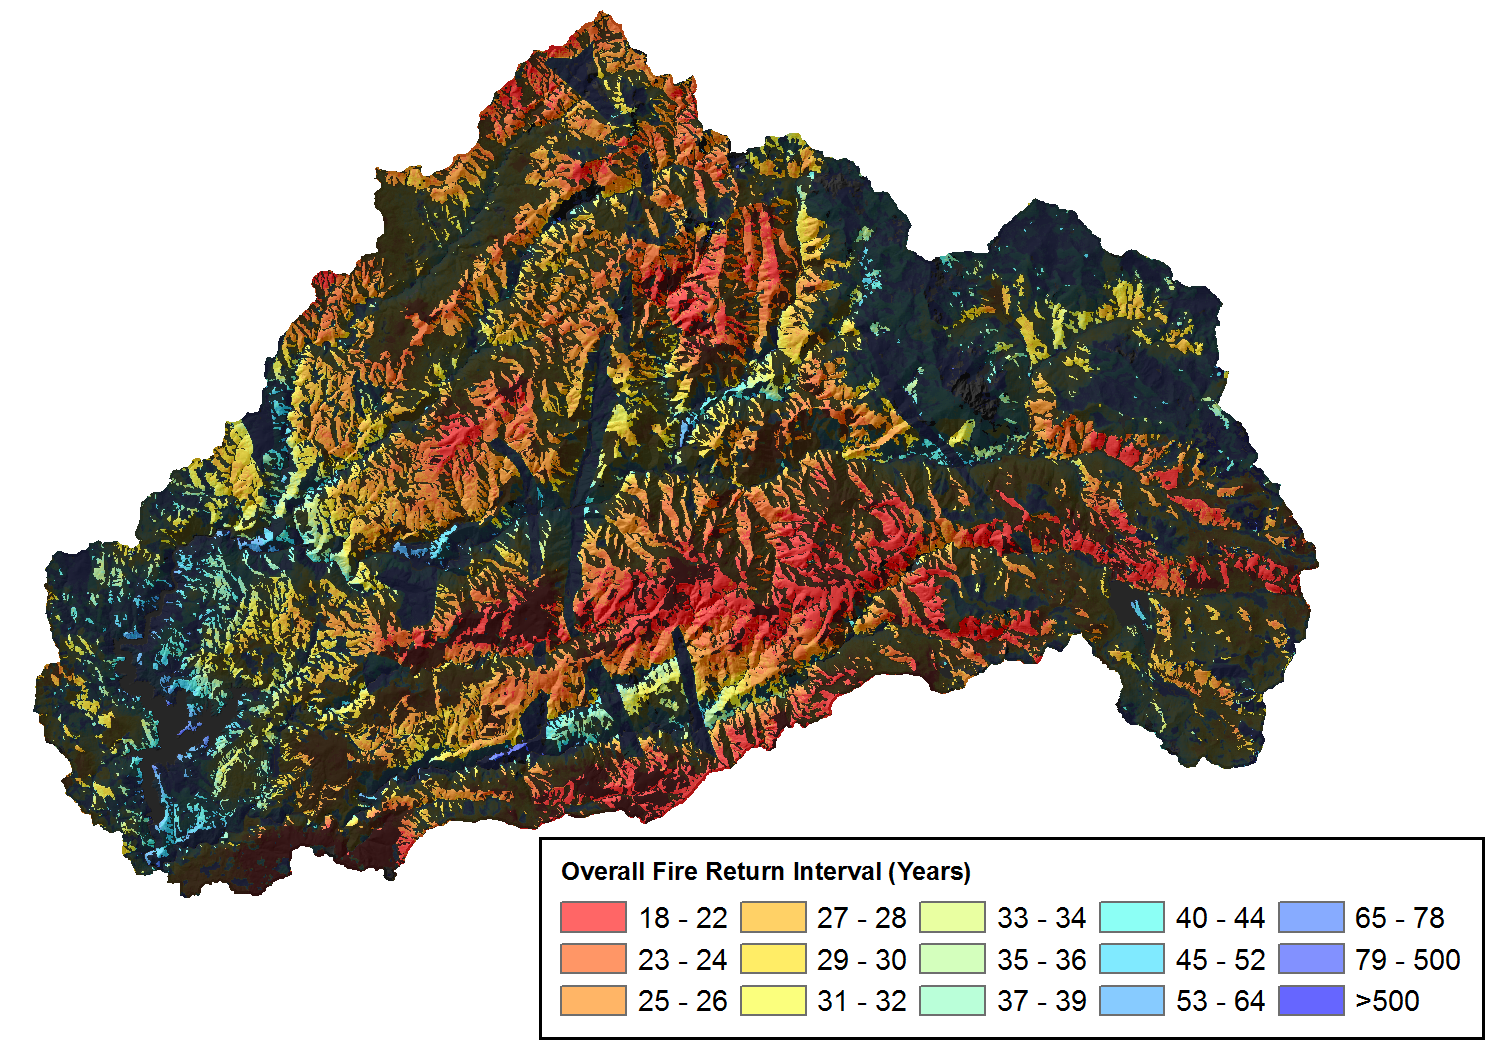
\includegraphics[width=0.5\textwidth]{/Users/mmallek/Tahoe/Report2/images/fri_smcx.png}
    }
  \caption{(a) Population return interval (average number of years between fires) distribution for Sierran Mixed Conifer - Xeric.  (b) Spatial depiction of fire return intervals across the landscape. Cover types other than Sierran Mixed Conifer - Xeric are partially obscured in grey. The value at any given cell is the point-specific return interval, which ranges from 17 years to \textgreater 500 years.}
\label{fig:preturn_smcx}
\end{figure}

\clearpage

%%%%%%%%%%%%%%%%%%%%%%%%%%%%%%%%
%%%%%%%%%%%%%%%%%%%%%%%%%%%%%%%%
%%%%%%%%%%%%%%%%%%%%%%%%%%%%%%%%
%\pagebreak[4]
\subsection{Vegetation Response}
\label{subsec:HRVvegresponse}

\subsubsection{Condition Sequence}\todo{these have been fixed}

Condition classes for each cover type varied over time. Evidence of both high mortality fire, which triggers a transition to early development conditions for all cover types, and low mortality fire, which can thin a stand and cause a transition to a more open canopy condition (within the same developmental stage), are visible in examining the output grids. Figure \ref{fig:covcondmaps} illustrates these changes for a sequence of four timesteps during the simulation.

\begin{figure}[!htbp]
  \centering
  \subfloat[][]{
    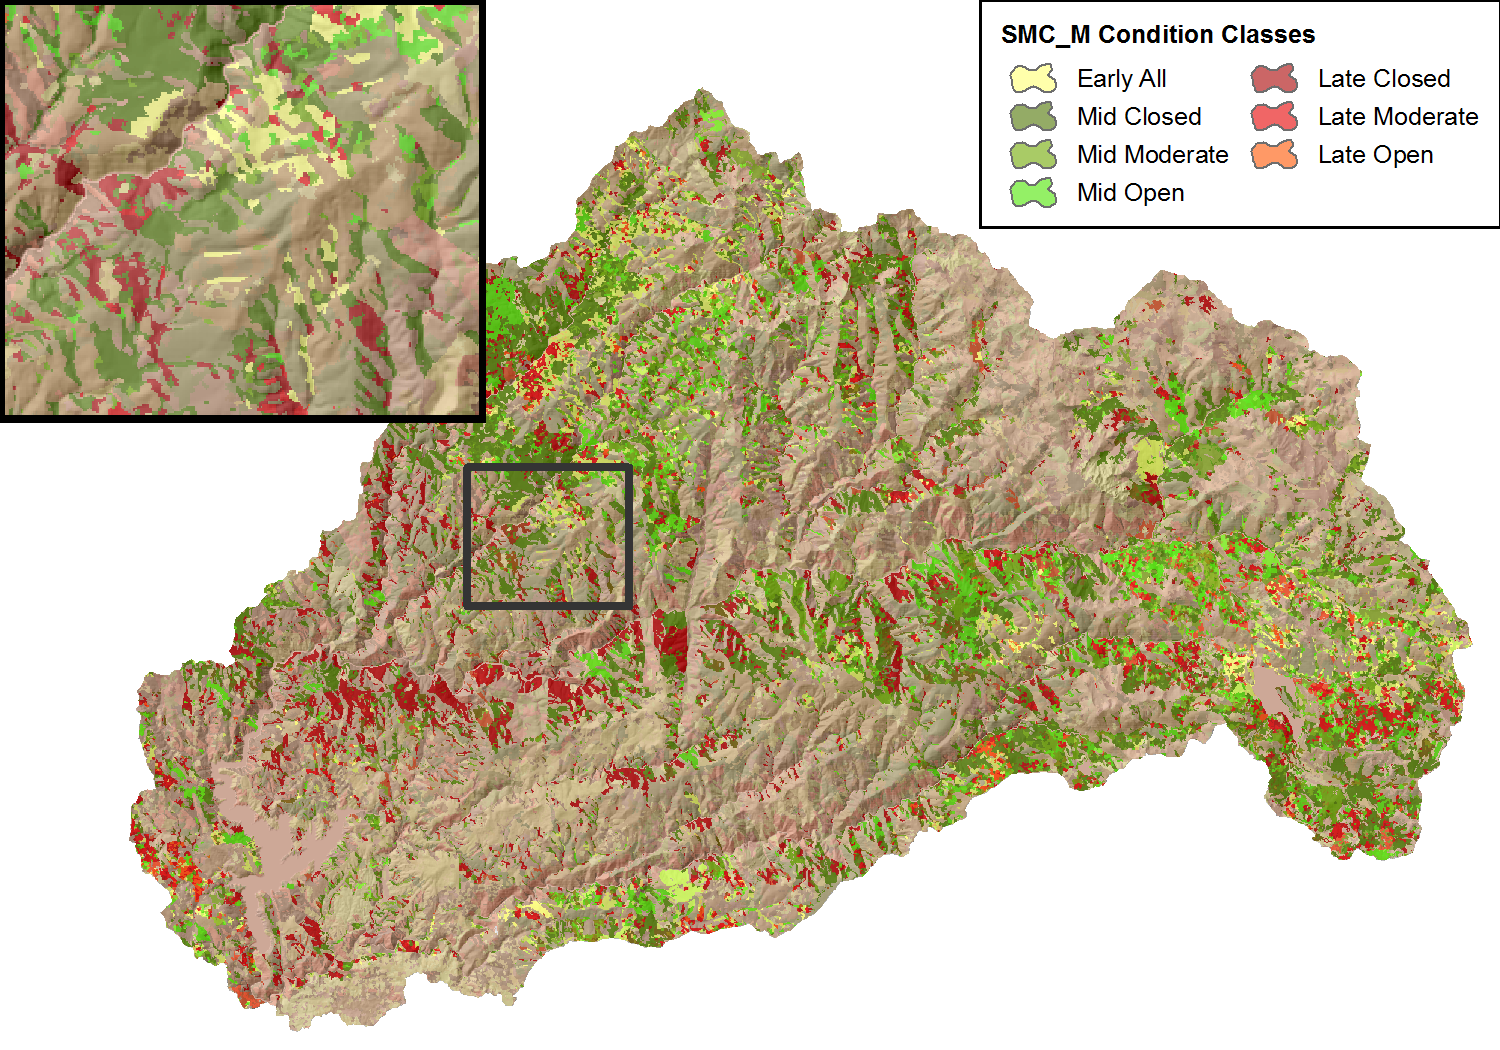
\includegraphics[width=0.5\textwidth]{/Users/mmallek/Tahoe/Report2/images/covcond660.png}
  }%
  \subfloat[][]{
    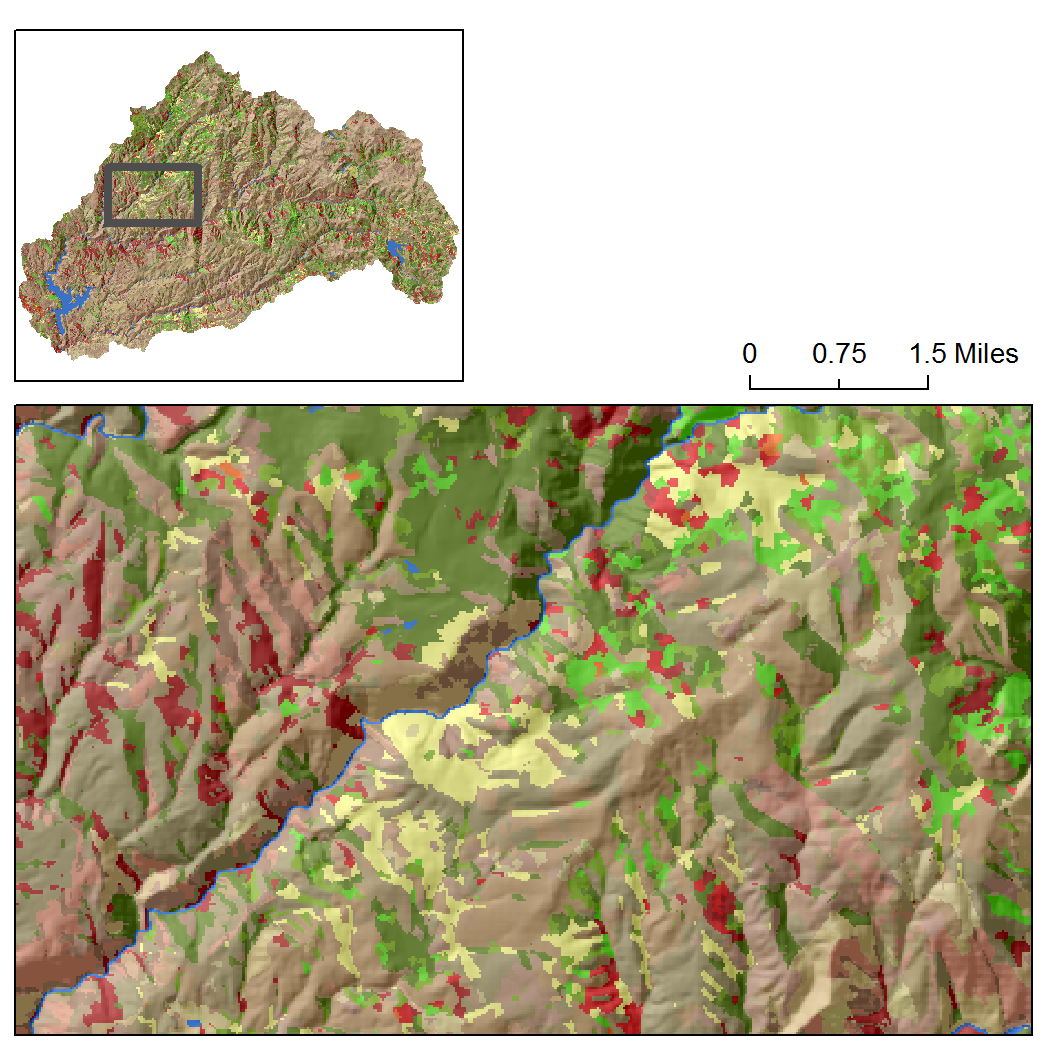
\includegraphics[width=0.5\textwidth]{/Users/mmallek/Tahoe/Report2/images/covcond665.png}
  }\\%
  \subfloat[][]{
    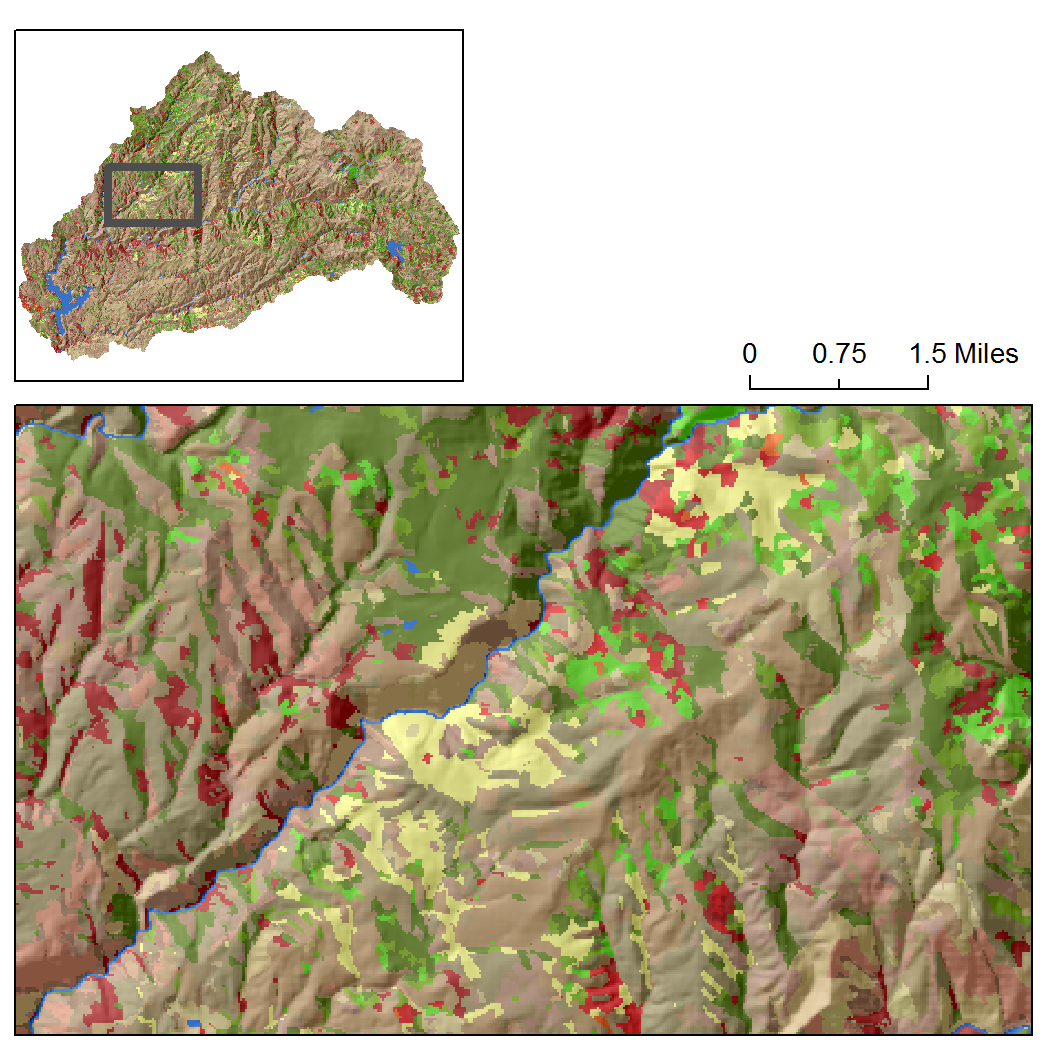
\includegraphics[width=0.5\textwidth]{/Users/mmallek/Tahoe/Report2/images/covcond670.png}
    }
  \subfloat[][]{
    \centering
    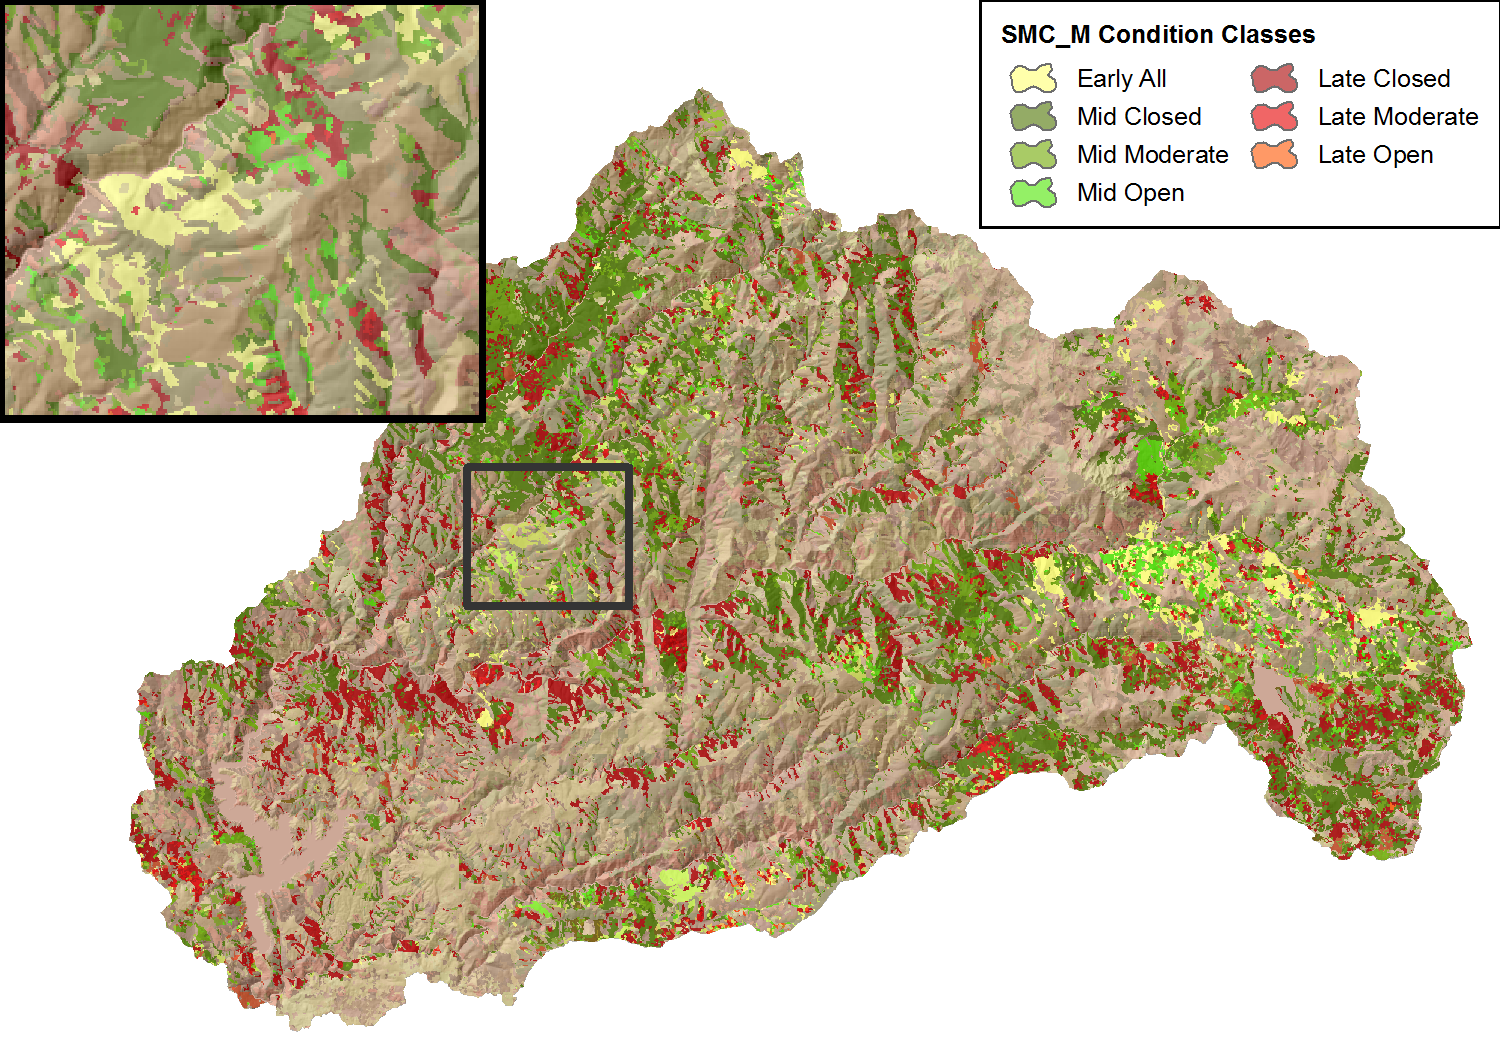
\includegraphics[width=0.5\textwidth]{/Users/mmallek/Tahoe/Report2/images/covcond675.png}
  }%
  \caption{A sequence of four timesteps during the simulation, showing changes in condition classes over time. Here we highlight the dominant cover type, Sierran Mixed Conifer - Mesic, and its classes, in order to illustrate the dynamics that play out over many years. (a) Timestep 660 (b) Timestep 665 (c) Timestep 670 (d) Timestep 675.}
  \label{fig:covcondmaps}
\end{figure}




\subsubsection{Landscape Composition} \todo{when I redid the plots I did them starting at year 40. should probably redo them with the line added in. can probably modify rmlstats call to do this.}

The distribution of area among condition classes within all cover types fluctuated over time, as expected. The relative proportion of each condition class also varied across cover types. In general, the condition class distribution appeared to be in dynamic equilibrium, despite considerable variability from timestep to timestep. The exception is the Oak-Conifer Forest and Woodland cover type, which did not appear to reach equilibrium until around timestep 220. The cover-condition dynamics and current seral stage distribution plots specific to each of the nine focal cover types follow (Figures \ref{fig:covcond_megm} through \ref{fig:covcond_smcx}).

% moved paragraph about general patterns to discussion


\todo{all these plots are redone}
\begin{figure}[!htbp]
  \centering
  \subfloat[][]{
    \centering
    \includegraphics[width=0.6\textwidth]{/Users/mmallek/Tahoe/R/Rplots/November2014/covcond_megm.png}
    }%
  \subfloat[][]{
  \centering
  \includegraphics[height=2.65in]{/Users/mmallek/Tahoe/R/Rplots/November2014/covcond_current_megm.png}
    }
  \caption{(a) Cover-Condition dynamics for Mixed Evergreen - Mesic. The black vertical line at 40 timesteps marks the end of the equilibration period used in this study. (b) Current seral stage distribution for Mixed Evergreen - Mesic.}
\label{fig:covcond_megm}
\end{figure}

%\clearpage

\begin{figure}[!htbp]
  \centering
  \subfloat[][]{
    \centering
    \includegraphics[width=0.6\textwidth]{/Users/mmallek/Tahoe/R/Rplots/November2014/covcond_megx.png}
    }%
  \subfloat[][]{
    \includegraphics[height=2.65in]{/Users/mmallek/Tahoe/R/Rplots/November2014/covcond_current_megx.png}
    }
  \caption{(a) Cover-Condition dynamics for Mixed Evergreen - Xeric. The black vertical line at 40 timesteps marks the end of the equilibration period used in this study. (b) Current seral stage distribution for Mixed Evergreen - Xeric.} 
  \label{fig:covcond_megx}
\end{figure}

\begin{figure}[!htbp]
  \centering
  \subfloat[][]{
    \centering
    \includegraphics[width=0.6\textwidth]{/Users/mmallek/Tahoe/R/Rplots/November2014/covcond_ocfw.png}
    }%
  \subfloat[][]{
    \includegraphics[height=2.65in]{/Users/mmallek/Tahoe/R/Rplots/November2014/covcond_current_ocfw.png}
    }
  \caption{(a) Cover-Condition dynamics for Oak-Conifer Forest and Woodland. The black vertical line at 40 timesteps marks the end of the equilibration period used in this study. (b) Current seral stage distribution for Oak-Conifer Forest and Woodland.} 
  \label{fig:covcond_ocfw}
\end{figure}

\begin{figure}[!htbp]
  \centering
  \subfloat[][]{
    \centering
    \includegraphics[width=0.6\textwidth]{/Users/mmallek/Tahoe/R/Rplots/November2014/covcond_ocfwu.png}
    }%
  \subfloat[][]{
    \includegraphics[height=2.65in]{/Users/mmallek/Tahoe/R/Rplots/November2014/covcond_current_ocfwu.png}
    }
  \caption{(a) Cover-Condition dynamics for Oak-Conifer Forest and Woodland - Ultramafic. The black vertical line at 40 timesteps marks the end of the equilibration period used in this study. (b) Current seral stage distribution for Oak-Conifer Forest and Woodland - Ultramafic.} 
  \label{fig:covcond_ocfwu}
\end{figure}

\begin{figure}[!htbp]
  \centering
  \subfloat[][]{
    \centering
    \includegraphics[width=0.6\textwidth]{/Users/mmallek/Tahoe/R/Rplots/November2014/covcond_rfrm.png}
    }%
  \subfloat[][]{
    \includegraphics[height=2.65in]{/Users/mmallek/Tahoe/R/Rplots/November2014/covcond_current_rfrm.png}
    }
  \caption{(a) Cover-Condition dynamics for Red Fir - Mesic. The black vertical line at 40 timesteps marks the end of the equilibration period used in this study. (b) Current seral stage distribution for Red Fir - Mesic.} 
  \label{fig:covcond_rfrm}
\end{figure}

\begin{figure}[!htbp]
  \centering
  \subfloat[][]{
    \centering
    \includegraphics[width=0.6\textwidth]{/Users/mmallek/Tahoe/R/Rplots/November2014/covcond_rfrx.png}
    }%
  \subfloat[][]{
    \includegraphics[height=2.65in]{/Users/mmallek/Tahoe/R/Rplots/November2014/covcond_current_rfrx.png}
    }
  \caption{(a) Cover-Condition dynamics for Red Fir - Xeric. The black vertical line at 40 timesteps marks the end of the equilibration period used in this study. (b) Current seral stage distribution for Red Fir - Xeric.} 
  \label{fig:covcond_rfrx}
\end{figure}

\begin{figure}[!htbp]
  \centering
  \subfloat[][]{
    \centering
    \includegraphics[width=0.6\textwidth]{/Users/mmallek/Tahoe/R/Rplots/November2014/covcond_smcm.png}
    }%
  \subfloat[][]{
    \includegraphics[height=2.65in]{/Users/mmallek/Tahoe/R/Rplots/November2014/covcond_current_smcm.png}
    }
  \caption{(a) Cover-Condition dynamics for Sierran Mixed Conifer - Mesic. The black vertical line at 40 timesteps marks the end of the equilibration period used in this study. (b) Current seral stage distribution for Sierran Mixed Conifer - Mesic.} 
  \label{fig:covcond_smcm}
\end{figure}

\begin{figure}[!htbp]
  \centering
  \subfloat[][]{
    \centering
    \includegraphics[width=0.6\textwidth]{/Users/mmallek/Tahoe/R/Rplots/November2014/covcond_smcu.png}
    }%
  \subfloat[][]{
    \includegraphics[height=2.65in]{/Users/mmallek/Tahoe/R/Rplots/November2014/covcond_current_smcu.png}
    }
  \caption{(a) Cover-Condition dynamics for Sierran Mixed Conifer - Ultramafic. The black vertical line at 40 timesteps marks the end of the equilibration period used in this study. (b) Current seral stage distribution for Sierran Mixed Conifer - Ultramafic.} 
  \label{fig:covcond_smcu}
\end{figure}

\begin{figure}[!htbp]
  \centering
  \subfloat[][]{
    \centering
    \includegraphics[width=0.6\textwidth]{/Users/mmallek/Tahoe/R/Rplots/November2014/covcond_smcx.png}
    }%
  \subfloat[][]{
    \includegraphics[height=2.65in]{/Users/mmallek/Tahoe/R/Rplots/November2014/covcond_current_smcx.png}
    }
  \caption{(a) Cover-Condition dynamics for Sierran Mixed Conifer - Xeric. The black vertical line at 40 timesteps marks the end of the equilibration period used in this study. (b) Current seral stage distribution for Sierran Mixed Conifer - Xeric.} 
  \label{fig:covcond_smcx}
\end{figure}



\todo{the covcond table has been redone}
\begin{landscape}
\begin{table}[!htbp]
\caption{Range of variation in landscape structure, illustrating the cover-condition class dynamics for Mixed Evergreen - Mesic (\textsc{meg\_m}), Mixed Evergreen - Xeric (\textsc{meg\_x}), Oak-Conifer Forest and Woodland (\textsc{ocfw}), and Oak-Conifer Forest and Woodland - Ultramafic (\textsc{ocfw\_u}). For condition class abbreviations, see Table \ref{condtable}.}
\label{tab:covcond1}
\begin{tabular}{@{}rrrrrrrrrr|rrr@{}}
\toprule
\footnotesize \textbf{\begin{tabular}[c]{@{}l@{}}Land \\ Cover\\ Type\end{tabular}} & \footnotesize \textbf{\begin{tabular}[c]{@{}l@{}}Condition \\ Class\end{tabular}} & \footnotesize \textbf{srv0\%} & \footnotesize \textbf{srv5\%} & \footnotesize \textbf{srv25\%} & \footnotesize \textbf{srv50\%} & \footnotesize \textbf{srv75\%} & \footnotesize \textbf{srv95\%} & \footnotesize \textbf{srv100\%}   & \footnotesize \textbf{\begin{tabular}[c]{@{}l@{}}Current\\ \%cover\end{tabular}} & \textbf{\begin{tabular}[c]{@{}l@{}}Current\\ \%srv\end{tabular}} & \textbf{\begin{tabular}[c]{@{}l@{}}Departure\\ Index\end{tabular}} \\ \midrule
\footnotesize \textsc{meg\_m}      & \footnotesize \textsc{early\_all}                & \footnotesize 0.22          & \footnotesize 1.19           & \footnotesize 2.13             & \footnotesize 3.21            & \footnotesize 4.67            & \footnotesize 7.27            & \footnotesize 10.05      & \footnotesize 8.21     & \footnotesize 97     & \footnotesize 94    \\
\footnotesize \textsc{meg\_m}      & \footnotesize \textsc{mid\_cl   }                & \footnotesize 0             & \footnotesize 0.01           & \footnotesize 0.09             & \footnotesize 0.32            & \footnotesize 0.79            & \footnotesize 2.17            & \footnotesize 8.01       & \footnotesize 36.53    & \footnotesize 100    & \footnotesize 100    \\
\footnotesize \textsc{meg\_m}      & \footnotesize \textsc{mid\_mod  }                & \footnotesize 0.15          & \footnotesize 0.67           & \footnotesize 1.25             & \footnotesize 2.09            & \footnotesize 3.41            & \footnotesize 5.57            & \footnotesize 9.15       & \footnotesize 9.76     & \footnotesize 100    & \footnotesize 100    \\
\footnotesize \textsc{meg\_m}      & \footnotesize \textsc{mid\_op   }                & \footnotesize 0             & \footnotesize 0.03           & \footnotesize 0.09             & \footnotesize 0.17            & \footnotesize 0.31            & \footnotesize 0.64            & \footnotesize 1.34       & \footnotesize 6.37     & \footnotesize 100    & \footnotesize 100    \\
\footnotesize \textsc{meg\_m}      & \footnotesize \textsc{late\_cl  }                & \footnotesize 48.42         & \footnotesize 56.9           & \footnotesize 66.822           & \footnotesize 72.96           & \footnotesize 78.05           & \footnotesize 83.01           & \footnotesize 89.6       & \footnotesize 29.31    & \footnotesize 0      & \footnotesize -100    \\
\footnotesize \textsc{meg\_m}      & \footnotesize \textsc{late\_mod }                & \footnotesize 4.2           & \footnotesize 8.08           & \footnotesize 10.84            & \footnotesize 13.69           & \footnotesize 16.62           & \footnotesize 20.88           & \footnotesize 23.51      & \footnotesize 7.31     & \footnotesize 2      & \footnotesize -96    \\
\footnotesize \textsc{meg\_m}      & \footnotesize \textsc{late\_op  }                & \footnotesize 1.16          & \footnotesize 2.42           & \footnotesize 4.68             & \footnotesize 6.51            & \footnotesize 9.49            & \footnotesize 14.26           & \footnotesize 18.14      & \footnotesize 2.5      & \footnotesize 6      & \footnotesize -88    \\
\footnotesize \textsc{meg\_x}      & \footnotesize \textsc{early\_all}                & \footnotesize 0.27          & \footnotesize 1.65           & \footnotesize 2.96             & \footnotesize 4.13            & \footnotesize 5.42            & \footnotesize 7.92            & \footnotesize 11.47      & \footnotesize 10.88    & \footnotesize 100    & \footnotesize 100    \\
\footnotesize \textsc{meg\_x}      & \footnotesize \textsc{mid\_cl   }                & \footnotesize 0             & \footnotesize 0.01           & \footnotesize 0.1              & \footnotesize 0.35            & \footnotesize 0.9             & \footnotesize 2.04            & \footnotesize 5.61       & \footnotesize 48.8     & \footnotesize 100    & \footnotesize 100    \\
\footnotesize \textsc{meg\_x}      & \footnotesize \textsc{mid\_mod  }                & \footnotesize 0.16          & \footnotesize 1.02           & \footnotesize 1.77             & \footnotesize 2.72            & \footnotesize 3.78            & \footnotesize 5.54            & \footnotesize 9.6        & \footnotesize 9.39     & \footnotesize 100    & \footnotesize 100    \\
\footnotesize \textsc{meg\_x}      & \footnotesize \textsc{mid\_op   }                & \footnotesize 0             & \footnotesize 0.03           & \footnotesize 0.14             & \footnotesize 0.27            & \footnotesize 0.45            & \footnotesize 0.9             & \footnotesize 1.69       & \footnotesize 12.87    & \footnotesize 100    & \footnotesize 100    \\
\footnotesize \textsc{meg\_x}      & \footnotesize \textsc{late\_cl  }                & \footnotesize 47.02         & \footnotesize 54.98          & \footnotesize 63.428           & \footnotesize 68.88           & \footnotesize 74.35           & \footnotesize 79.78           & \footnotesize 89.32      & \footnotesize 12.84    & \footnotesize 0      & \footnotesize -100    \\
\footnotesize \textsc{meg\_x}      & \footnotesize \textsc{late\_mod }                & \footnotesize 6.15          & \footnotesize 10.25          & \footnotesize 13.55            & \footnotesize 16.11           & \footnotesize 18.63           & \footnotesize 22.85           & \footnotesize 25.76      & \footnotesize 3.84     & \footnotesize 0      & \footnotesize -100    \\
\footnotesize \textsc{meg\_x}      & \footnotesize \textsc{late\_op  }                & \footnotesize 1.51          & \footnotesize 2.92           & \footnotesize 4.81             & \footnotesize 6.78            & \footnotesize 9.17            & \footnotesize 12.77           & \footnotesize 16.4       & \footnotesize 1.38     & \footnotesize 0      & \footnotesize -100    \\
\footnotesize \textsc{ocfw}        & \footnotesize \textsc{early\_all}                & \footnotesize 1.99          & \footnotesize 6.37           & \footnotesize 10.022           & \footnotesize 12.88           & \footnotesize 16.6            & \footnotesize 21.92           & \footnotesize 28.04      & \footnotesize 19.97    & \footnotesize 90     & \footnotesize 80    \\
\footnotesize \textsc{ocfw}        & \footnotesize \textsc{mid\_cl   }                & \footnotesize 1.22          & \footnotesize 3.84           & \footnotesize 8.188            & \footnotesize 11.9            & \footnotesize 15.76           & \footnotesize 20.18           & \footnotesize 28.33      & \footnotesize 37.36    & \footnotesize 100    & \footnotesize 100    \\
\footnotesize \textsc{ocfw}        & \footnotesize \textsc{mid\_mod  }                & \footnotesize 4.37          & \footnotesize 6.25           & \footnotesize 8.333            & \footnotesize 9.9             & \footnotesize 11.94           & \footnotesize 16.43           & \footnotesize 19.88      & \footnotesize 14.61    & \footnotesize 91     & \footnotesize 82    \\
\footnotesize \textsc{ocfw}        & \footnotesize \textsc{mid\_op   }                & \footnotesize 3.51          & \footnotesize 6.9            & \footnotesize 10.05            & \footnotesize 13.13           & \footnotesize 17.23           & \footnotesize 21.88           & \footnotesize 26.49      & \footnotesize 24.34    & \footnotesize 100    & \footnotesize 100    \\
\footnotesize \textsc{ocfw}        & \footnotesize \textsc{late\_cl  }                & \footnotesize 3.08          & \footnotesize 7.01           & \footnotesize 13.996           & \footnotesize 20.56           & \footnotesize 27.04           & \footnotesize 34.97           & \footnotesize 43.7       & \footnotesize 1.58     & \footnotesize 0      & \footnotesize -100    \\
\footnotesize \textsc{ocfw}        & \footnotesize \textsc{late\_mod }                & \footnotesize 10.5          & \footnotesize 13.58          & \footnotesize 16.387           & \footnotesize 18.4            & \footnotesize 20.7            & \footnotesize 24.13           & \footnotesize 27.77      & \footnotesize 1.02     & \footnotesize 0      & \footnotesize -100    \\
\footnotesize \textsc{ocfw}        & \footnotesize \textsc{late\_op  }                & \footnotesize 2.33          & \footnotesize 4.73           & \footnotesize 7.62             & \footnotesize 10.54           & \footnotesize 14.17           & \footnotesize 19.16           & \footnotesize 25.48      & \footnotesize 1.12     & \footnotesize 0      & \footnotesize -100    \\
\footnotesize \textsc{ocfw\_u}     & \footnotesize \textsc{early\_all}                & \footnotesize 0.64          & \footnotesize 1.2            & \footnotesize 1.92             & \footnotesize 2.91            & \footnotesize 4.07            & \footnotesize 8.01            & \footnotesize 15.1       & \footnotesize 17.76    & \footnotesize 100    & \footnotesize 100    \\
\footnotesize \textsc{ocfw\_u}     & \footnotesize \textsc{mid\_cl   }                & \footnotesize 0.01          & \footnotesize 0.01           & \footnotesize 0.02             & \footnotesize 0.03            & \footnotesize 0.09            & \footnotesize 0.28            & \footnotesize 2.21       & \footnotesize 29.32    & \footnotesize 100    & \footnotesize 100    \\
\footnotesize \textsc{ocfw\_u}     & \footnotesize \textsc{mid\_mod  }                & \footnotesize 0.06          & \footnotesize 0.17           & \footnotesize 0.44             & \footnotesize 0.74            & \footnotesize 1.55            & \footnotesize 3.5             & \footnotesize 7.07       & \footnotesize 11.54    & \footnotesize 100    & \footnotesize 100    \\
\footnotesize \textsc{ocfw\_u}     & \footnotesize \textsc{mid\_op   }                & \footnotesize 1.07          & \footnotesize 1.72           & \footnotesize 3.07             & \footnotesize 4.58            & \footnotesize 7.04            & \footnotesize 12.31           & \footnotesize 16.93      & \footnotesize 33.49    & \footnotesize 100    & \footnotesize 100    \\
\footnotesize \textsc{ocfw\_u}     & \footnotesize \textsc{late\_cl  }                & \footnotesize 0.12          & \footnotesize 0.12           & \footnotesize 0.15             & \footnotesize 0.16            & \footnotesize 0.2             & \footnotesize 0.61            & \footnotesize 2.36       & \footnotesize 5.35     & \footnotesize 100    & \footnotesize 100    \\
\footnotesize \textsc{ocfw\_u}     & \footnotesize \textsc{late\_mod }                & \footnotesize 0.39          & \footnotesize 0.59           & \footnotesize 1.22             & \footnotesize 1.66            & \footnotesize 2.96            & \footnotesize 10.01           & \footnotesize 17.65      & \footnotesize 2.2      & \footnotesize 64     & \footnotesize 28    \\
\footnotesize \textsc{ocfw\_u}     & \footnotesize \textsc{late\_op  }                & \footnotesize 52.73         & \footnotesize 71.22          & \footnotesize 85.27            & \footnotesize 88.54           & \footnotesize 91.3            & \footnotesize 94.05           & \footnotesize 94.57      & \footnotesize 0.34     & \footnotesize 0      & \footnotesize -100    \\
\end{tabular}
\end{table}
\end{landscape}


\begin{landscape}
\begin{table}[!htbp]
\caption{Range of variation in landscape structure, illustrating the cover-condition class dynamics for Red Fir - Mesic (\textsc{rfr\_m}), Red Fir - Xeric (\textsc{rfr\_x}), Sierran Mixed Conifer - Mesic (\textsc{smc\_m}), and Sierran Mixed Conifer - Ultramafic (\textsc{smc\_u}). For condition class abbreviations, see Table \ref{condtable}.}
\label{tab:covcond2}
\begin{tabular}{@{}lllllllllllll@{}}
\toprule
\footnotesize \textbf{\begin{tabular}[c]{@{}l@{}}Land \\ Cover\\ Type\end{tabular}} & \footnotesize \textbf{\begin{tabular}[c]{@{}l@{}}Condition \\ Class\end{tabular}} & \footnotesize \textbf{srv0\%} & \footnotesize \textbf{srv5\%} & \footnotesize \textbf{srv25\%} & \footnotesize \textbf{srv50\%} & \footnotesize \textbf{srv75\%} & \footnotesize \textbf{srv95\%} & \footnotesize \textbf{srv100\%}   & \footnotesize \textbf{\begin{tabular}[c]{@{}l@{}}Current\\ \%cover\end{tabular}} & \textbf{\begin{tabular}[c]{@{}l@{}}Current\\ \%srv\end{tabular}} & \textbf{\begin{tabular}[c]{@{}l@{}}Departure\\ Index\end{tabular}} \\ \midrule
\footnotesize \textsc{rfr\_m}      & \footnotesize \textsc{early\_all}               & \footnotesize 3.35           & \footnotesize  6.47           & \footnotesize 10.66            & \footnotesize 15.55            & \footnotesize 21.42            & \footnotesize 31.77            & \footnotesize 53.6        & \footnotesize 24.21    & \footnotesize 82      & \footnotesize 64    \\
\footnotesize \textsc{rfr\_m}      & \footnotesize \textsc{mid\_cl   }               & \footnotesize 8.45           & \footnotesize  18.13          & \footnotesize 26.4             & \footnotesize 33.9             & \footnotesize 40.44            & \footnotesize 51.99            & \footnotesize 58.87       & \footnotesize 3.63     & \footnotesize 0       & \footnotesize -100    \\
\footnotesize \textsc{rfr\_m}      & \footnotesize \textsc{mid\_mod  }               & \footnotesize 0.38           & \footnotesize  0.65           & \footnotesize 1.04             & \footnotesize 1.38             & \footnotesize 1.82             & \footnotesize 2.67             & \footnotesize 3.03        & \footnotesize 18.67    & \footnotesize 100     & \footnotesize 100    \\
\footnotesize \textsc{rfr\_m}      & \footnotesize \textsc{mid\_op   }               & \footnotesize 0.13           & \footnotesize  0.3            & \footnotesize 0.57             & \footnotesize 0.82             & \footnotesize 1.32             & \footnotesize 2.29             & \footnotesize 2.98        & \footnotesize 16.7     & \footnotesize 100     & \footnotesize 100    \\
\footnotesize \textsc{rfr\_m}      & \footnotesize \textsc{late\_cl  }               & \footnotesize 20.21           & \footnotesize 26.48          & \footnotesize 32.96            & \footnotesize 39.64            & \footnotesize 46.45            & \footnotesize 60.84            & \footnotesize 71.22       & \footnotesize 10.7     & \footnotesize 0       & \footnotesize -100    \\
\footnotesize \textsc{rfr\_m}      & \footnotesize \textsc{late\_mod }               & \footnotesize 1.02           & \footnotesize  1.53           & \footnotesize 2.32             & \footnotesize 3.04             & \footnotesize 3.9              & \footnotesize 5.46             & \footnotesize 7.59        & \footnotesize 21.96    & \footnotesize 100     & \footnotesize 100    \\
\footnotesize \textsc{rfr\_m}      & \footnotesize \textsc{late\_op  }               & \footnotesize 0.68           & \footnotesize  1.14           & \footnotesize 1.99             & \footnotesize 2.91             & \footnotesize 4.12             & \footnotesize 6.59             & \footnotesize 9.34        & \footnotesize 4.13     & \footnotesize 76      & \footnotesize 52    \\
\footnotesize \textsc{rfr\_x}      & \footnotesize \textsc{early\_all}               & \footnotesize 16.16           & \footnotesize 21.18          & \footnotesize 30.17            & \footnotesize 35.64            & \footnotesize 41.28            & \footnotesize 46.36            & \footnotesize 50.38       & \footnotesize 32.39    & \footnotesize 34      & \footnotesize -32    \\
\footnotesize \textsc{rfr\_x}      & \footnotesize \textsc{mid\_cl   }               & \footnotesize 0.08           & \footnotesize  0.31           & \footnotesize 0.66             & \footnotesize 1.14             & \footnotesize 2.09             & \footnotesize 4.46             & \footnotesize 8.99        & \footnotesize 8.26     & \footnotesize 100     & \footnotesize 100    \\
\footnotesize \textsc{rfr\_x}      & \footnotesize \textsc{mid\_mod  }               & \footnotesize 2.12           & \footnotesize  3.72           & \footnotesize 6.09             & \footnotesize 8.39             & \footnotesize 10.8             & \footnotesize 14.74            & \footnotesize 19.8        & \footnotesize 18.66    & \footnotesize 100     & \footnotesize 100    \\
\footnotesize \textsc{rfr\_x}      & \footnotesize \textsc{mid\_op   }               & \footnotesize 7.88           & \footnotesize  11.82          & \footnotesize 16.21            & \footnotesize 19.85            & \footnotesize 23.45            & \footnotesize 27.63            & \footnotesize 31.38       & \footnotesize 12.58    & \footnotesize 8       & \footnotesize -84    \\
\footnotesize \textsc{rfr\_x}      & \footnotesize \textsc{late\_cl  }               & \footnotesize 6.9            & \footnotesize  8.99           & \footnotesize 12.6             & \footnotesize 15.37            & \footnotesize 19.29            & \footnotesize 26.44            & \footnotesize 35.67       & \footnotesize 10.45    & \footnotesize 10      & \footnotesize -80    \\
\footnotesize \textsc{rfr\_x}      & \footnotesize \textsc{late\_mod }               & \footnotesize 6.32           & \footnotesize  8.07           & \footnotesize 9.66             & \footnotesize 10.81            & \footnotesize 12.3             & \footnotesize 14.64            & \footnotesize 16.78       & \footnotesize 14.57    & \footnotesize 95      & \footnotesize 90    \\
\footnotesize \textsc{rfr\_x}      & \footnotesize \textsc{late\_op  }               & \footnotesize 1.44           & \footnotesize  4.44           & \footnotesize 6.08             & \footnotesize 7.5              & \footnotesize 8.96             & \footnotesize 11.57            & \footnotesize 14.96       & \footnotesize 3.1      & \footnotesize 2       & \footnotesize -96    \\
\footnotesize \textsc{smc\_m}      & \footnotesize \textsc{early\_all}               & \footnotesize 1.72           & \footnotesize  7.01           & \footnotesize 10.39            & \footnotesize 13.99            & \footnotesize 17.25            & \footnotesize 21.2             & \footnotesize 29.33       & \footnotesize 14.98    & \footnotesize 56      & \footnotesize 12    \\
\footnotesize \textsc{smc\_m}      & \footnotesize \textsc{mid\_cl   }               & \footnotesize 6.92           & \footnotesize  11.56          & \footnotesize 15.98            & \footnotesize 19.74            & \footnotesize 23.75            & \footnotesize 28.8             & \footnotesize 37.13       & \footnotesize 9.74     & \footnotesize 3       & \footnotesize -94    \\
\footnotesize \textsc{smc\_m}      & \footnotesize \textsc{mid\_mod  }               & \footnotesize 4.71           & \footnotesize  6.54           & \footnotesize 8.48             & \footnotesize 10.07            & \footnotesize 12.23            & \footnotesize 16.38            & \footnotesize 21.72       & \footnotesize 17.97    & \footnotesize 97      & \footnotesize 94    \\
\footnotesize \textsc{smc\_m}      & \footnotesize \textsc{mid\_op   }               & \footnotesize 4.39           & \footnotesize  9.46           & \footnotesize 12.86            & \footnotesize 16.27            & \footnotesize 19.86            & \footnotesize 25.74            & \footnotesize 31.18       & \footnotesize 16.29    & \footnotesize 51      & \footnotesize 2    \\
\footnotesize \textsc{smc\_m}      & \footnotesize \textsc{late\_cl  }               & \footnotesize 2.28           & \footnotesize  5.22           & \footnotesize 10.07            & \footnotesize 14.61            & \footnotesize 19.18            & \footnotesize 24.25            & \footnotesize 29.97       & \footnotesize 23.23    & \footnotesize 93      & \footnotesize 86    \\
\footnotesize \textsc{smc\_m}      & \footnotesize \textsc{late\_mod }               & \footnotesize 8.06           & \footnotesize  9.53           & \footnotesize 11.04            & \footnotesize 12.3             & \footnotesize 14.08            & \footnotesize 17.26            & \footnotesize 23.44       & \footnotesize 14.18    & \footnotesize 77      & \footnotesize 54    \\
\footnotesize \textsc{smc\_m}      & \footnotesize \textsc{late\_op  }               & \footnotesize 2.64           & \footnotesize  5.72           & \footnotesize 8.31             & \footnotesize 11.04            & \footnotesize 14.04            & \footnotesize 17.76            & \footnotesize 22.74       & \footnotesize 3.6      & \footnotesize 1       & \footnotesize -98    \\
\footnotesize \textsc{smc\_u}      & \footnotesize \textsc{early\_all}               & \footnotesize 15.18          & \footnotesize  22.8           & \footnotesize 28.15            & \footnotesize 31.51            & \footnotesize 34.69            & \footnotesize 38.5             & \footnotesize 42.79       & \footnotesize 48.7     & \footnotesize 100     & \footnotesize 100    \\
\footnotesize \textsc{smc\_u}      & \footnotesize \textsc{mid\_cl   }               & \footnotesize 0.19           & \footnotesize  0.37           & \footnotesize 0.61             & \footnotesize 0.81             & \footnotesize 1.15             & \footnotesize 1.78             & \footnotesize 3.26        & \footnotesize 2.99     & \footnotesize 100     & \footnotesize 100    \\
\footnotesize \textsc{smc\_u}      & \footnotesize \textsc{mid\_mod  }               & \footnotesize 3.02           & \footnotesize  3.84           & \footnotesize 5.06             & \footnotesize 6.45             & \footnotesize 8.19             & \footnotesize 10.82            & \footnotesize 13.15       & \footnotesize 6.77     & \footnotesize 54      & \footnotesize 8    \\
\footnotesize \textsc{smc\_u}      & \footnotesize \textsc{mid\_op   }               & \footnotesize 18.21          & \footnotesize  21.22          & \footnotesize 23.99            & \footnotesize 26.16            & \footnotesize 28.91            & \footnotesize 31.96            & \footnotesize 38.31       & \footnotesize 5.33     & \footnotesize 0       & \footnotesize -100    \\
\footnotesize \textsc{smc\_u}      & \footnotesize \textsc{late\_cl  }               & \footnotesize 5.95           & \footnotesize  7.84           & \footnotesize 10.16            & \footnotesize 12.6             & \footnotesize 15.36            & \footnotesize 20.31            & \footnotesize 26.89       & \footnotesize 24.43    & \footnotesize 99      & \footnotesize 98    \\
\footnotesize \textsc{smc\_u}      & \footnotesize \textsc{late\_mod }               & \footnotesize 6.87           & \footnotesize  8.91           & \footnotesize 9.91             & \footnotesize 10.87            & \footnotesize 12.19            & \footnotesize 14.84            & \footnotesize 21.19       & \footnotesize 8.51     & \footnotesize 2       & \footnotesize -96    \\
\footnotesize \textsc{smc\_u}      & \footnotesize \textsc{late\_op  }               & \footnotesize 4.29           & \footnotesize  6.36           & \footnotesize 8.48             & \footnotesize 10.19            & \footnotesize 12.24            & \footnotesize 15.85            & \footnotesize 20.96       & \footnotesize 3.27     & \footnotesize 0       & \footnotesize -100    \\
\end{tabular}
\end{table}
\end{landscape}


\begin{landscape}
\begin{table}[!htbp]
\caption{Range of variation in landscape structure, illustrating the cover-condition class dynamics for Sierran Mixed Conifer -~Xeric (\textsc{smc\_x}). For condition class abbreviations, see Table \ref{condtable}.}
\label{tab:covcond3}
\begin{tabular}{@{}lllllllllllll@{}}
\toprule
\footnotesize \textbf{\begin{tabular}[c]{@{}l@{}}Land \\ Cover\\ Type\end{tabular}} & \footnotesize \textbf{\begin{tabular}[c]{@{}l@{}}Condition \\ Class\end{tabular}} & \footnotesize \textbf{srv0\%} & \footnotesize \textbf{srv5\%} & \footnotesize \textbf{srv25\%} & \footnotesize \textbf{srv50\%} & \footnotesize \textbf{srv75\%} & \footnotesize \textbf{srv95\%} & \footnotesize \textbf{srv100\%}   & \footnotesize \textbf{\begin{tabular}[c]{@{}l@{}}Current\\ \%cover\end{tabular}} & \textbf{\begin{tabular}[c]{@{}l@{}}Current\\ \%srv\end{tabular}} & \textbf{\begin{tabular}[c]{@{}l@{}}Departure\\ Index\end{tabular}} \\ \midrule
\footnotesize \textsc{smc\_x}      & \footnotesize \textsc{early\_all}     & \footnotesize 19.96           & \footnotesize 23.94           & \footnotesize 29.41            & \footnotesize 34.33            & \footnotesize 40.07            & \footnotesize 44.49           & \footnotesize 47.42        & \footnotesize 19.48    & \footnotesize 0    & \footnotesize -100     \\
\footnotesize \textsc{smc\_x}      & \footnotesize \textsc{mid\_cl   }     & \footnotesize 0.05           & \footnotesize 0.11           & \footnotesize 0.3            & \footnotesize 0.58            & \footnotesize 1.08            & \footnotesize 1.84           & \footnotesize 3.6        & \footnotesize 11.96    & \footnotesize 100    & \footnotesize 100     \\
\footnotesize \textsc{smc\_x}      & \footnotesize \textsc{mid\_mod  }     & \footnotesize 2.28           & \footnotesize 4.2           & \footnotesize 6.35            & \footnotesize 8.36            & \footnotesize 10.39            & \footnotesize 13.79           & \footnotesize 18.2        & \footnotesize 14.92    & \footnotesize 98    & \footnotesize 96     \\
\footnotesize \textsc{smc\_x}      & \footnotesize \textsc{mid\_op   }     & \footnotesize 19.43           & \footnotesize 23.87           & \footnotesize 26.72            & \footnotesize 29.57            & \footnotesize 32.27            & \footnotesize 35.47           & \footnotesize 40.86        & \footnotesize 11.48    & \footnotesize 0    & \footnotesize -100     \\
\footnotesize \textsc{smc\_x}      & \footnotesize \textsc{late\_cl  }     & \footnotesize 0.44           & \footnotesize 1.45           & \footnotesize 3.15            & \footnotesize 5.08            & \footnotesize 7.36            & \footnotesize 10.36           & \footnotesize 13.31        & \footnotesize 24.72    & \footnotesize 100    & \footnotesize 100     \\
\footnotesize \textsc{smc\_x}      & \footnotesize \textsc{late\_mod }     & \footnotesize 4.65           & \footnotesize 5.65           & \footnotesize 7.29            & \footnotesize 8.58            & \footnotesize 9.98            & \footnotesize 12.86           & \footnotesize 16.61        & \footnotesize 13.31    & \footnotesize 98    & \footnotesize 96     \\
\footnotesize \textsc{smc\_x}      & \footnotesize \textsc{late\_op  }     & \footnotesize 2.91           & \footnotesize 7.05           & \footnotesize 9.86            & \footnotesize 12.24            & \footnotesize 14.94            & \footnotesize 17.42           & \footnotesize 19.81        & \footnotesize 4.13    & \footnotesize 1    & \footnotesize -98     \\ \bottomrule 
\end{tabular}
\end{table}
\end{landscape}



\clearpage
\pagebreak[4]
\subsubsection{Landscape Configuration}
We summarize the structure and patterns in the landscape using a suite of statistical measures calculated using \textsc{Fragstats}. Table \ref{tab:fragland} shows the range of variability for the simulation period as well as the current value and depature index. Patch density and patch richness are within the simulated HRV, but the other fifteen metrics are outside the 5$^{\text{th}}$ to 95$^{\text{th}}$ percentile range of variability. See Section \ref{subsec:dataanalysis} for a detailed description of \textsc{Fragstats} metrics.
\todo{this section of text updated}
The departure index indicates the distance from the 50$^{\text{th}}$ percentile value for a given metric. It is computed by subtracting 50 from the current value's percentile (if that value is between 0 and 50) under the simulated range of variability (SRV) then dividing by 50 and multiplying by 100 (to ensure the departure index scales from 0 to 100). Thus, for the landscape metric \emph{Patch Density}, 19.507 is equivalent to the 32$^{\text{nd}}$ percentile of observations during the HRV simulation, and the departure index is $(39-50)/50*100 = -22$). This value is within the HRV for the landscape. However, the landscape metric \emph{Edge Density} is 100, because $128.875 > 125.316$, the largest value observed during the HRV simulation. Edge density at the landscape level is outside the HRV.

One of the principal purposes of gaining a better quantitative understanding of the historic reference period is to know whether recent human activities have caused landscapes to move outside their historic range of variability (Landres et al.1999, Swetnam et al. 1999). As described above, we summarized the distribution of each metric calculated over the length of the simulation, minus the equilibration period. We computed the 0$^{\text{th}}$, 5$^{\text{th}}$, 25$^{\text{th}}$, 50$^{\text{th}}$, 75$^{\text{th}}$, 95$^{\text{th}}$ and 100$^{\text{th}}$ percentiles of the distribution of observed values. The current percentile for the statistical range of variability refers to the place within the 0--100$^{\text{th}}$ percentile of the observed, simulated HRV. If the current value is outside the HRV, it is given the appropriate maximum (100) or minimum (0) score. The index of departure from HRV measures the relative distance from the median HRV value to the 0$^{\text{th}}$ or 100$^{\text{th}}$ percentile. At the landscape-level, most computed metrics have values outside the HRV. 

Several of the individual landscape metrics are redundant with one another. For example, \emph{Contagion} and \emph{Edge Density} are inversely related, so it is perhaps helpful, but not necessary, to examine both metrics. In Figures \ref{fig:fragland_areashape}, \ref{fig:fragland_contagsiei}, and \ref{fig:fragland_core} we highlight a subset of the metrics from Table \ref{tab:fragland} for the purposes of discussing the landscape under the simulated historic period as compared to the present day. Figures for all metrics are included in \todo{the appendix?}.

\todo{this table updated}
\begin{landscape}
\begin{table}[!htbp]
\caption{NEW DEPARTURE INDEX! Range of variability during the simulation for a selected suite of landscape configuration metrics calculated using \textsc{Fragstats}. The landscape metrics listed here are described in detail in the 
\textsc{Fragstats} methods section. 
\textsc{pd} = patch density; 
\textsc{ed} = edge density; 
\textsc{area\_am} = area-weighted mean patch size; 
\textsc{gyrate\_am} = area-weighted mean patch radius of gyration (correlation length); 
\textsc{shape\_am} = area-weighted mean patch shape index; 
\textsc{core\_am} = area-weighted mean patch core area; 
\textsc{cai\_am} = area-weighted mean patch core area index; 
\textsc{simi\_mn} = mean similarity; 
\textsc{cwed} = contrast-weighted edge density; 
\textsc{teci} = total edge contrast index; 
\textsc{econ\_am} = area-weighted mean edge contrast; 
\textsc{contag} = contagion; 
\textsc{iji} = interspersion and juxtaposition index; 
\textsc{pr} = patch richness; 
\textsc{sidi} = Simpson's diversity index; 
\textsc{siei} = Simpson's evenness index; 
\textsc{ai} = aggregation index.}
\label{tab:fragland}
\begin{tabular}{@{}llllllll|lll@{}}
\toprule
\textbf{\begin{tabular}[c]{@{}l@{}}Landscape\\ Metric\end{tabular}} & \textbf{srv0\%} & \textbf{srv5\%} & \textbf{srv25\%} & \textbf{srv50\%} & \textbf{srv75\%} & \textbf{srv95\%} & \textbf{srv100\%}  & \textbf{\begin{tabular}[c]{@{}l@{}}Current\\ Value\end{tabular}} & \textbf{\begin{tabular}[c]{@{}l@{}}Current\\ \%SRV\end{tabular}} & \textbf{\begin{tabular}[c]{@{}l@{}}Departure\\ Index\end{tabular}} \\ \midrule
\small \textsc{pd}              & 18.308       & 18.823      & 19.206        & 19.463       & 19.684        & 20.017        & 20.47         & 19.507      & 55     & 4    \\
\small \textsc{ed}              & 117.074       & 117.619      & 118.835        & 119.558       & 120.347        & 121.199        & 123.358         & 128.875      & 100     & 245    \\
\small \textsc{area\_am}        & 158.508       & 167.738      & 177.762        & 188.395       & 199.899        & 212.94        & 231.284         & 119.985      & 0     & -229     \\
\small \textsc{gyrate\_am}      & 703.538       & 714.365      & 727.305        & 740.046       & 754.819        & 773.62        & 808.962         & 620.951      & 0     & -326     \\
\small \textsc{shape\_am}       & 3.614       & 3.648      & 3.707        & 3.751       & 3.812        & 3.874        & 4         & 3.243      & 0     & -371     \\
\small \textsc{core\_am}        & 132.831       & 143.938      & 154.408        & 164.025       & 175.058        & 188.071        & 209.479         & 106.71      & 0     & -184     \\
\small \textsc{cai\_am}         & 61.425       & 62.88      & 63.838        & 64.875       & 65.832        & 67.104        & 68.272         & 65.295      & 62     & 12   \\
\small \textsc{simi\_mn}        & 2272.713       & 2434.457      & 2587.924        & 2691.305       & 2814.235        & 3013.224        & 3263.13         & 2095.764      & 0     & -142     \\
\small \textsc{cwed}            & 37.992       & 38.503      & 38.91        & 39.3       & 39.71        & 40.405        & 41.416         & 36.092      & 0     & -245     \\
\small \textsc{teci}            & 31.224       & 31.662      & 32.091        & 32.418       & 32.815        & 33.479        & 34.024         & 27.654      & 0     & -399     \\
\small \textsc{econ\_am}        & 31.165       & 31.662      & 32.107        & 32.42       & 32.857        & 33.567        & 34.203         & 27.756      & 0     & -372     \\
\small \textsc{contag}          & 52.273       & 52.95      & 53.407        & 53.775       & 54.154        & 54.797        & 55.593         & 51.172      & 0     & -173     \\
\small \textsc{iji }            & 62.508       & 63.501      & 64.328        & 64.766       & 65.176        & 65.848        & 66.597         & 65.868      & 96     & 60    \\
\small \textsc{pr}              & 109       & 114      & 117        & 118       & 120        & 122        & 124         & 117      & 24     & -11    \\
\small \textsc{sidi}            & 0.94       & 0.946      & 0.95        & 0.953       & 0.955        & 0.958        & 0.96         & 0.962      & 100     & 129    \\
\small \textsc{siei}            & 0.948       & 0.954      & 0.958        & 0.961       & 0.963        & 0.966        & 0.968         & 0.971      & 100     & 143    \\
\small \textsc{ai}              & 81.755       & 82.081      & 82.211        & 82.329       & 82.439        & 82.614        & 82.707         & 80.963      & 0     & -238     \\ \bottomrule
\end{tabular}
\end{table}
\end{landscape}


\clearpage
\todo{these plots have been redone}
\begin{figure}[!htbp]
  \centering
  \subfloat[][]{
    \centering
\includegraphics[width=0.5\textwidth]{/Users/mmallek/Tahoe/R/Rplots/November2014/AREA_AM1.png}
    }%
  \subfloat[][]{
\includegraphics[width=0.5\textwidth]{/Users/mmallek/Tahoe/R/Rplots/November2014/SHAPE_AM1.png}
  }
\caption{Landscape \textsc{Fragstats} Metrics. Left, Area-weighted Mean Patch Area. Right, Area-weighted Mean Shape. We use the area-weighted metrics to reduce the influence of the many extremely small patches. The average patch size is larger, and the average patch shape more complex, than the current landscape.} 
\label{fig:fragland_areashape}
\end{figure}

\begin{figure}[!htbp]
  \centering
  \subfloat[][]{
    \centering
\includegraphics[width=0.5\textwidth]{/Users/mmallek/Tahoe/R/Rplots/November2014/CONTAG1.png}
    }%
  \subfloat[][]{
\includegraphics[width=0.5\textwidth]{/Users/mmallek/Tahoe/R/Rplots/November2014/SIEI1.png}
  }
\caption{Landscape \textsc{Fragstats} Metrics. (a) Contagion, a metric describing patch dispersion and interspersion. The landscape during the HRV is much more contagious than the current landscape. (b) Simpson's Evenness Index, which indicates the distance from maximum diversity, or evenness, in the landscape patches. Values for Simpson's Evenness are near 1 during the HRV and in the present landscape, but the HRV values are well below the current conditions.} 
\label{fig:fragland_contagsiei}
\end{figure}

\begin{figure}[!htbp]
  \centering
  \includegraphics[width=0.5\textwidth]{/Users/mmallek/Tahoe/R/Rplots/November2014/CORE_AM1.png}
\caption{Landscape \textsc{Fragstats} Metrics. Results for the Area-weighted Mean Core Area, a measure of interior habitat available at the patch level. During the HRV, the average patch contains more core area than in the current landscape.} 
\label{fig:fragland_core}
\end{figure}


\section{Future Management Scenarios}